% -*- latex -*-
%
% The SAND document class is maintained at:
%
%    http://www.cs.sandia.gov/SANDreport
%
% This page also has instructions and documentation on commands.
%
\documentclass[12pt,report]{SANDreport}

\SANDnum{SAND20XX-XXXX}
\SANDprintDate{January 20XX}

\title{VTK-m Users' Guide \\
  \relsize{-2}Version 0.0
}
\author{Kenneth~Moreland \\
  \relsize{-2} Scalable Analysis and Visualization \\[-1ex]
  \relsize{-2} Sandia National Laboratories \\[-1ex]
  \relsize{-2} P.O. Box 5800 MS 1323 \\[-1ex]
  \relsize{-2} Albuquerque, NM 87185-1323 \\[-1ex]
  \relsize{-2} kmorel@sandia.gov
}
\SANDauthor{Kenneth~Moreland}
\date{} % Leave empty


\usepackage{amsfonts}
\usepackage{amssymb}
\usepackage{amsmath}
\usepackage{booktabs}
\usepackage{graphicx}
\usepackage{isomath}
\usepackage{varioref}
\usepackage{fancyvrb}
\usepackage{ifthen}
\usepackage{longtable}
\usepackage{cite}
\usepackage{relsize}
\usepackage{subfig}
\usepackage{xspace}

% This wonderful package allows hyphenation in tt fonts and hyphenation of
% words with underscores in them.
\usepackage[htt]{hyphenat}

% This package defines a tt font that supports boldface (albeit not very
% distinctly). The default package has no boldface for tt fonts.
\usepackage{lmodern}

\usepackage{makeidx}
\makeindex

\usepackage[pdfborder={0 0 0}]{hyperref}
\usepackage{verbatim}

\usepackage{color}
\definecolor{yellow}{rgb}{1,1,0}
\definecolor{black}{rgb}{0,0,0}
\definecolor{ltcyan}{rgb}{.75,1,1}
\definecolor{red}{rgb}{1,0,0}
\definecolor{gray}{rgb}{.6,.6,.6}
\definecolor{darkred}{rgb}{0.5,0,0}
\definecolor{darkgreen}{rgb}{0,0.5,0}

\definecolor{vtkmidentifier}{rgb}{0,0,1}
\definecolor{vtkmnamespace}{rgb}{0.5,0,0}
\definecolor{vtkmmacro}{rgb}{0.5,0,0}
\definecolor{vtkmsignature}{rgb}{0,0.5,0}

\usepackage{listings}
\lstloadlanguages{C,C++}
\lstset{fontadjust=false,basicstyle=\scriptsize\ttfamily}
%% \lstset{numbers=left, numberstyle=\tiny, stepnumber=1, numbersep=2pt}
\lstdefinelanguage{VTKm}{
  morekeywords={struct,class,public,typedef,void,template,return,operator,const,for,int},
  morekeywords={[2]Id,Id2,Id3,Scalar,Tuple,Vector2,Vector3,Vector4,
                   make_Id3,make_Vector2,make_Vector3,make_Vector4,
                   dot,NUM_COMPONENTS,
                   Extent,Extent3,Pair,
                   ExtentPointDimensions,ExtentCellDimensions,
                   ExtentNumberOfPoints,ExtentNumberOfCells,
                   ExtentPointFlatIndexToTopologyIndex,
                   ExtentCellFlatIndexToTopologyIndex,
                   ExtentPointTopologyIndexToFlatIndex,
                   ExtentCellTopologyIndexToFlatIndex,
                   ExtentFirstPointOnCell,
                   ListTagEmpty,
                   ListTagBase,ListTagBase2,ListTagBase3,ListTagBase4,
                   ListTagJoin,
                   ListForEach,
                   TypeListTagId,TypeListTagId2,TypeListTagId3,
                   TypeListTagScalar,
                   TypeListTagVector2,TypeListTagVector3,TypeListTagVector4,
                   TypeListTagIndex,TypeListTagReal,
                   TypeListTagAll,TypeListTagCommon,
                   WorkletMapField, WorkletMapCell,
                   WorkletGenerateTopology, WorkletInterpolatedCell,
                   WorkletGenerateKeysValues, WorkletReduceKeysValues,
                   ExecutionObjectBase,
                   TypeTraits,NumericTag,DimensionalityTag,
                   TypeTraitsRealTag,TypeTraitsIntegerTag,
                   TypeTraitsScalarTag,TypeTraitsVectorTag,
                   VectorTraits,ComponentType,HasMultipleComponents,
                   VectorTraitsTagMultipleComponents,
                   VectorTraitsTagSingleComponent,
                   Error, ErrorExecution, ErrorControl,
                   ErrorControlAssert, ErrorControlBadValue,
                   ErrorControlInternal, ErrorControlOutOfMemory,
                   DeviceAdapterTagSerial,
                   DeviceAdapterTagCuda,
                   DeviceAdapterTagOpenMP,
                   DeviceAdapterTagTBB,
                   CellAverage,
                   CellDataToPointDataGenerateKeys,CellDataToPointDataReduceKeys,
                   CellGradient,
                   Cosine,Sine,Magnitude,Square,
                   Elevation,
                   MarchingCubesClassify,MarchingCubesGenerate,
                   PointDataToCellData,
                   SliceClassify,SliceGenerate,
                   Tetrahedralize,
                   ThresholdClassify,ThresholdTopology,
                   ArrayHandle,make_ArrayHandle,
                   ArrayHandleConstant,make_ArrayHandleConstant,
                   ArrayHandleCounting,make_ArrayHandleCounting,
                   ArrayContainerControl,
                   ArrayContainerControlTagBasic,
                   ArrayContainerControlTagImplicit,
                   ArrayTransfer,
                   ArrayManagerExecution,
                   ArrayManagerExecutionShareWithControl,
                   DeviceAdapterAlgorithm, DeviceAdapterAlgorithmGeneral,
                   IteratorFromArrayPortal,
                   UniformGrid,UnstructuredGrid,
                   DispatcherMapField, DispatcherMapCell,
                   DispatcherGenerateTopology, DispatcherInterpolatedCell,
                   DispatcherGenerateKeysValues,
                   DispatcherReduceKeysValues,
                   CellField, CellVertices,
                   InterpolatedCellPoints,
                   CellTraits,NUM_VERTICES,
                   CellTagHexahedron, CellTagLine, CellTagQuadrilateral,
                   CellTagTetrahedron, CellTagTriangle, CellTagVectex,
                   CellTagVoxel, CellTagWedge,
                   CellTraits,
                   CellTopologicalDimensionsTag,
                   GridTagUniform, GridTagUnstructured,
                   NUM_VERTICES, TOPOLOGICAL_DIMENSIONS,
                   ParametricCoordinates, CellDerivative,
                   SortLess, SortGreater,
                   Max, Min,
                   Cbrt, Exp, Exp10, Exp2, ExpM1, Log, Log10, Log1P, Log2,
                   Pow, RCbrt, RSqrt, Sqrt,
                   Matrix, Matrix2x2, Matrix3x3, Matrix4x4,
                   MatrixColumn, MatrixDeterminant, MatrixIdentity,
                   MatrixInverse, MatrixMultiply, MatrixRow,
                   MatrixSetColumn, MatrixSetRow, MatrixTranspose,
                   SolveLinearSystem,
                   NewtonsMethod,
                   Ceil, Epsilon, Floor, FMod, Infinity, IsFinite, IsInf,
                   IsNan, ModF, Nan, NegativeInfinity, Remainder,
                   RemainderQuotient, Round,
                   Abs, CopySign, IsNegative, SignBit,
                   ACos, ACosH, ASin, ASinH, ATan, ATan2, ATanH, Cos, CosH,
                   Pi, Sin, SinH, Tan, TanH,
                   Cross, Magnitude, MagnitudeSquared, Lerp, Normal,
                   Normalize, RMagnitude, TriangleNormal,
                   ParametricCoordinatesToWorldCoordinates,
                   WorldCoordinatesToParametricCoordinates,
                   ParametricCoordinates,
                   TransferToOpenGL
                   },
  morekeywords={[3]VTKM_CONT_EXPORT,VTKM_EXEC_EXPORT,VTKM_EXEC_CONT_EXPORT,
                   VTKM_EXEC_CONSTANT_EXPORT,
                   VTKM_DEVICE_ADAPTER,
                   VTKM_DEVICE_ADAPTER_SERIAL,
                   VTKM_DEVICE_ADAPTER_CUDA,
                   VTKM_DEVICE_ADAPTER_OPENMP,
                   VTKM_DEVICE_ADAPTER_TBB,
                   VTKM_DEVICE_ADAPTER_ERROR,
                   VTKM_DEFAULT_DEVICE_ADAPTER_TAG,
                   VTKM_ARRAY_CONTAINER_CONTROL,
                   VTKM_ARRAY_CONTAINER_CONTROL_BASIC,
                   VTKM_ARRAY_CONTAINER_CONTROL_ERROR,
                   VTKM_DEFAULT_ARRAY_CONTAINER_CONTROL_TAG,
                   VTKM_ASSERT_CONT,
                   VTKM_DEFAULT_TYPE_LIST_TAG
                   },
  morekeywords={[4]vtkm,exec,cont,worklet,math,cuda,openmp,tbb,internal,detail},
  morekeywords={[5]ControlSignature, ExecutionSignature,
                   Field,Topology,Geometry,
                   In,Out,Point,Cell,Vertices,Values,KeyGroup,ExecObject,
                   WorkId,VisitIndex,
                   _1,_2,_3,_4,_5,_6,_7,_8,_9
                   }
}
\lstset{language=VTKm}
\lstset{
  keywordstyle=\bfseries,
  keywordstyle=[2]\color{vtkmidentifier},
  keywordstyle=[3]\color{vtkmmacro},
  keywordstyle=[4]\color{vtkmnamespace},
  keywordstyle=[5]\color{vtkmsignature}
}

\renewcommand{\lstlistlistingname}{List of Examples}
\renewcommand{\lstlistingname}{Example}

\newcommand*{\textcode}[1]{\texttt{#1}}
\newcommand*{\textnamespace}[1]{\textcode{\color{vtkmnamespace}{#1}}}
\newcommand*{\textmacro}[1]{\textcode{\color{vtkmmacro}{#1}}}
\newcommand*{\textidentifier}[1]{\textcode{\color{vtkmidentifier}{#1}}}
\newcommand*{\textsignature}[1]{\textcode{\color{vtkmsignature}{#1}}}

\newcommand*{\vtkmmacro}[1]{\textmacro{#1}\index{#1}}

\newcommand{\vtkmcontexport}{\vtkmmacro{VTKM\_CONT\_EXPORT}\index{export!control}\index{function~export}\index{method~export}\xspace}
\newcommand{\vtkmexecexport}{\vtkmmacro{VTKM\_EXEC\_EXPORT}\index{export!execution}\index{function~export}\index{method~export}\xspace}
\newcommand{\vtkmexeccontexport}{\vtkmmacro{VTKM\_EXEC\_CONT\_EXPORT}\index{export!control}\index{export!execution}\index{function~export}\index{method~export}\xspace}

\newcommand{\controlsignature}{\textsignature{ControlSignature}\index{control~signature}\index{signature!control}\xspace}
\newcommand{\executionsignature}{\textsignature{ExecutionSignature}\index{execution~signature}\index{signature!execution}\xspace}

\newcommand*{\sigtag}[1]{\textsignature{#1}\index{#1}\index{signature tags!#1}}
\newcommand*{\sigtagnum}[1]{\sigtag{\_#1}}
\newcommand*{\sigtagmod}[2]{\sigtag{#1}\textcode{(}\sigtag{#2}\textcode{)}}
\newcommand*{\sigtagmodnum}[2]{\sigtag{#1}\textcode{(}\sigtagnum{#2}\textcode{)}}

\newcommand*{\writenamespaceone}[1]{%
  \textnamespace{#1}}
\newcommand*{\writenamespacetwo}[2]{%
  \writenamespaceone{#1}\textcode{:\colonhyp}\textnamespace{#2}}
\newcommand*{\writenamespacethree}[3]{%
  \writenamespacetwo{#1}{#2}\textcode{:\colonhyp}\textnamespace{#3}}
\newcommand*{\writenamespacefour}[4]{%
  \writenamespacethree{#1}{#2}{#3}\textcode{:\colonhyp}\textnamespace{#4}}

\newcommand*{\indexnamespaceone}[1]{%
  \index{#1 namespace}\index{namespace!#1}}
\newcommand*{\indexnamespacetwo}[2]{%
  \index{#2 namespace}\index{#1::#2}\index{namespace!#1::#2}}
\newcommand*{\indexnamespacethree}[3]{%
  \index{#3 namespace}\index{#1::#2::#3}\index{namespace!#1::#2::#3}}
\newcommand*{\indexnamespacefour}[4]{%
  \index{#4 namespace}\index{#1::#2::#3::#4}\index{namespace!#1::#2::#3::#4}}

\newcommand*{\writeindexidentifierone}[2]{%
  \writenamespaceone{#1}\textcode{:\colonhyp}\textidentifier{#2}%
  \index{#2}}
\newcommand*{\writeindexidentifiertwo}[3]{%
  \writenamespacetwo{#1}{#2}\textcode{:\colonhyp}\textidentifier{#3}%
  \index{#3}}
\newcommand*{\writeindexidentifierthree}[4]{%
  \writenamespacethree{#1}{#2}{#3}\textcode{:\colonhyp}\textidentifier{#4}%
  \index{#4}}
\newcommand*{\writeindexidentifierfour}[5]{%
  \writenamespacefour{#1}{#2}{#3}{#4}\textcode{:\colonhyp}\textidentifier{#5}%
  \index{#5}}

\newcommand*{\vtkm}[1]{%
  \ifthenelse{\equal{#1}{}}%
             {\writenamespaceone{vtkm}\indexnamespaceone{vtkm}}%
             {\writeindexidentifierone{vtkm}{#1}}}
\newcommand*{\vtkmcont}[1]{%
  \ifthenelse{\equal{#1}{}}%
             {\writenamespacetwo{vtkm}{cont}\indexnamespacetwo{vtkm}{cont}}%
             {\writeindexidentifiertwo{vtkm}{cont}{#1}}}
\newcommand*{\vtkmcontinternal}[1]{%
  \ifthenelse{\equal{#1}{}}%
             {\writenamespacethree{vtkm}{cont}{internal}\indexnamespacethree{vtkm}{cont}{internal}}%
             {\writeindexidentifierthree{vtkm}{cont}{internal}{#1}}}
\newcommand*{\vtkmexec}[1]{%
  \ifthenelse{\equal{#1}{}}%
             {\writenamespacetwo{vtkm}{exec}\indexnamespacetwo{vtkm}{exec}}%
             {\writeindexidentifiertwo{vtkm}{exec}{#1}}}
\newcommand*{\vtkmexecinternal}[1]{%
  \ifthenelse{\equal{#1}{}}%
             {\writenamespacethree{vtkm}{exec}{internal}\indexnamespacethree{vtkm}{cont}{internal}}%
             {\writeindexidentifierthree{vtkm}{exec}{internal}{#1}}}
\newcommand*{\vtkmworklet}[1]{%
  \ifthenelse{\equal{#1}{}}%
             {\writenamespacetwo{vtkm}{worklet}\indexnamespacetwo{vtkm}{worklet}}%
             {\writeindexidentifiertwo{vtkm}{worklet}{#1}}}
\newcommand*{\vtkmmath}[1]{%
  \ifthenelse{\equal{#1}{}}%
             {\writenamespacetwo{vtkm}{math}\indexnamespacetwo{vtkm}{math}}%
             {\writeindexidentifiertwo{vtkm}{math}{#1}}}

\newcommand*{\vtkmcuda}[1]{%
  \ifthenelse{\equal{#1}{}}%
             {\writenamespacetwo{vtkm}{cuda}\indexnamespacetwo{vtkm}{cuda}}%
             {\writeindexidentifiertwo{vtkm}{cuda}{#1}}}
\newcommand*{\vtkmcudacont}[1]{%
  \ifthenelse{\equal{#1}{}}%
             {\writenamespacethree{vtkm}{cuda}{cont}\indexnamespacethree{vtkm}{cuda}{cont}}%
             {\writeindexidentifierthree{vtkm}{cuda}{cont}{#1}}}
\newcommand*{\vtkmopenmp}[1]{%
  \ifthenelse{\equal{#1}{}}%
             {\writenamespacetwo{vtkm}{openmp}\indexnamespacetwo{vtkm}{openmp}}%
             {\writeindexidentifiertwo{vtkm}{openmp}{#1}}}
\newcommand*{\vtkmopenmpcont}[1]{%
  \ifthenelse{\equal{#1}{}}%
             {\writenamespacethree{vtkm}{openmp}{cont}\indexnamespacethree{vtkm}{openmp}{cont}}%
             {\writeindexidentifierthree{vtkm}{openmp}{cont}{#1}}}
\newcommand*{\vtkmtbb}[1]{%
  \ifthenelse{\equal{#1}{}}%
             {\writenamespacetwo{vtkm}{tbb}\indexnamespacetwo{vtkm}{tbb}}%
             {\writeindexidentifiertwo{vtkm}{tbb}{#1}}}
\newcommand*{\vtkmtbbcont}[1]{%
  \ifthenelse{\equal{#1}{}}%
             {\writenamespacethree{vtkm}{tbb}{cont}\indexnamespacethree{vtkm}{tbb}{cont}}%
             {\writeindexidentifierthree{vtkm}{tbb}{cont}{#1}}}

\newcommand*{\vtkmopengl}[1]{%
  \ifthenelse{\equal{#1}{}}%
             {\writenamespacetwo{vtkm}{opengl}\indexnamespacetwo{vtkm}{opengl}}%
             {\writeindexidentifiertwo{vtkm}{opengl}{#1}}}

\newcommand*{\tparams}[1]{\textcode{<#1>}}

\newcommand*{\textfilename}[1]{\textsf{#1}}
\newcommand*{\vtkmheader}[2]{%
  \textfilename{#1\fshyp{}#2}\index{#1\fshyp#2}\index{#2}}

\newcommand*{\cmakevar}[1]{%
  \textsf{#1}%
  \index{#1}%
  \index{CMake configuration!#1}}

\lstnewenvironment{vtkmexample}[2][-*-]{
  \lstset{caption={#2}}
  \ifthenelse{\equal{#1}{-*-}}{}{\lstset{label=#1}}
}{
}

\newcommand*{\vtkmlisting}[3][]{
  \lstinputlisting[language=VTKm, label=#1, caption={#2}]{examples/listing_#3}
}

% Cite commands I use to abstract away the different ways to reference an
% entry in the bibliography (superscripts, numbers, dates, or author
% abbreviations).  \scite is a short cite that is used immediately after
% when the authors are mentioned.  \lcite is a full citation that is used
% anywhere.  Both should be used right next to the text being cited without
% any spacing.
\newcommand*{\lcite}[1]{~\cite{#1}}
\newcommand*{\scite}[1]{~\cite{#1}}

\newcommand{\etal}{et al.}

\newcommand*{\keyterm}[1]{\emph{#1}}

\newcommand{\fix}[1]{{\color{red}\textsc{[#1]}}}
%\newcommand{\fix}[1]{}

% Avoid putting figures on their own page.
\renewcommand{\textfraction}{0.05}
\renewcommand{\topfraction}{0.95}
\renewcommand{\bottomfraction}{0.95}

% Make sure this is big enough so that only big figures end up on their own
% page but small enough so that if a figure does have to be on its own
% page, it won't push everything to the bottom because it's not big enough
% to have its own page.
\renewcommand{\floatpagefraction}{.75}

% Environments for tightly packed lists.
\newenvironment{enumeratetight}{
  \begin{enumerate}
    \setlength{\topsep}{0pt}
    \setlength{\itemsep}{0pt}
    \setlength{\parskip}{0pt}
    \setlength{\parsep}{0pt}
    \setlength{\partopsep}{0pt}
}{
  \end{enumerate}
}

\newenvironment{itemizetight}{
  \begin{itemize}
    \setlength{\topsep}{0pt}
    \setlength{\itemsep}{0pt}
    \setlength{\parskip}{0pt}
    \setlength{\parsep}{0pt}
    \setlength{\partopsep}{0pt}
}{
  \end{itemize}
}

\newenvironment{descriptiontight}{
  \begin{description}
    \setlength{\topsep}{0pt}
    \setlength{\itemsep}{0pt}
    \setlength{\parskip}{0pt}
    \setlength{\parsep}{0pt}
    \setlength{\partopsep}{0pt}
}{
  \end{description}
}

\begin{document}

\sloppy

\maketitle

\begin{abstract}
  \fix{Write this.}
\end{abstract}

\clearpage

\chapter*{Acknowledgement}

\fix{Write this. Can steal from Dax document.}


\cleardoublepage % TOC should start on an odd page
\tableofcontents
\listoffigures
%\listoftables
\lstlistoflistings

\clearpage

\SANDmain

% -*- latex -*-

\chapter{Introduction}
\label{chap:Introduction}

High-performance computing relies on ever finer threading. Advances in
processor technology include ever greater numbers of cores, hyperthreading,
accelerators with integrated blocks of cores, and special vectorized
instructions, all of which require more software parallelism to achieve
peak performance. Traditional visualization solutions cannot support this
extreme level of concurrency. Extreme scale systems require a new
programming model and a fundamental change in how we design algorithms. To
address these issues we created VTK-m: the visualization toolkit for
multi-/many-core architectures.

VTK-m supports a number of algorithms and the ability to design further
algorithms through a top-down design with an emphasis on extreme
parallelism. VTK-m also provides support for finding and building links
across topologies, making it possible to perform operations that determine
manifold surfaces, interpolate generated values, and find adjacencies.
Although Dax provides a simplified high-level interface for programming,
its template-based code removes the overhead of abstraction.

\begin{figure}[htb]
  \centering
  \begin{tabular}{ccc}
    CUDA SDK & PISTON & VTK-m \\
    {\small 431 LOC} & {\small 369 LOC} & {\small 265 LOC} \\
    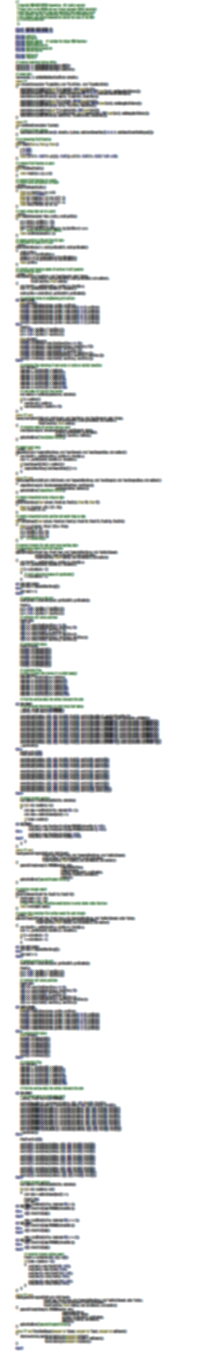
\includegraphics[width=.75in]{images/MCCompareCuda} &
    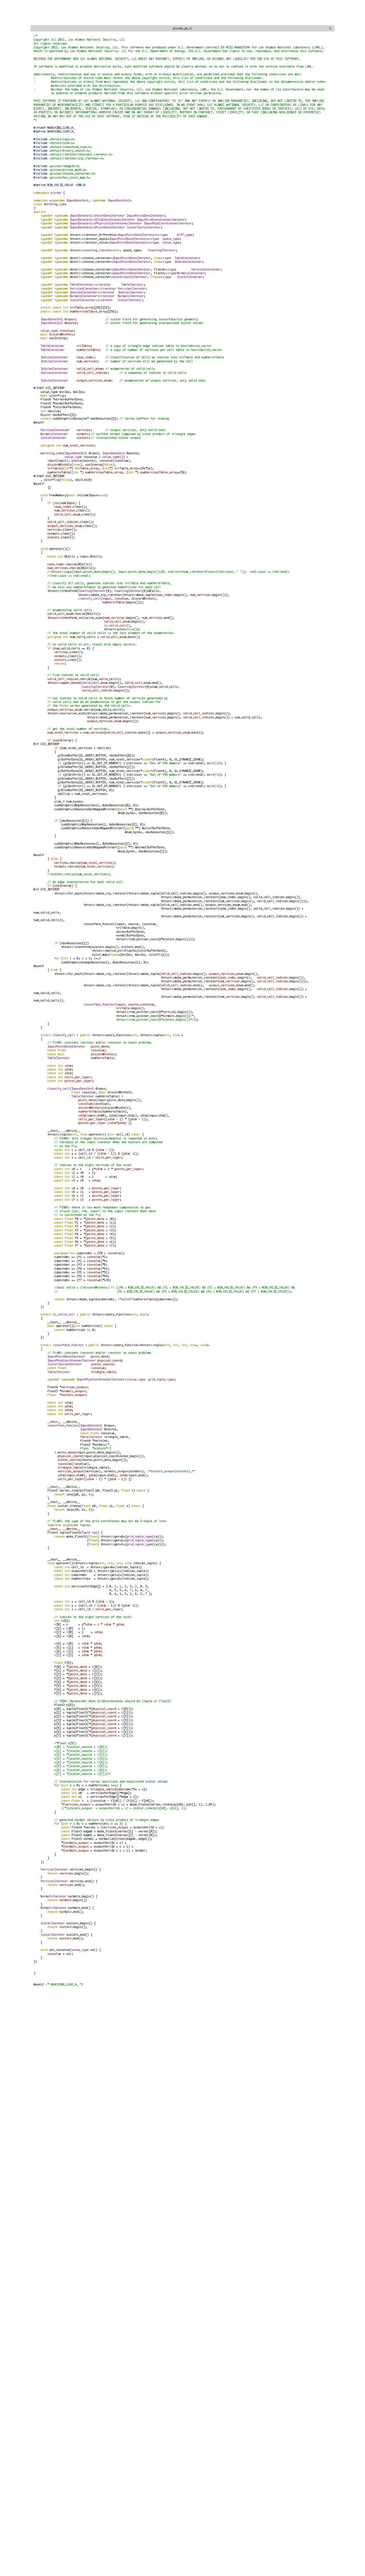
\includegraphics[width=.75in]{images/MCComparePiston} &
    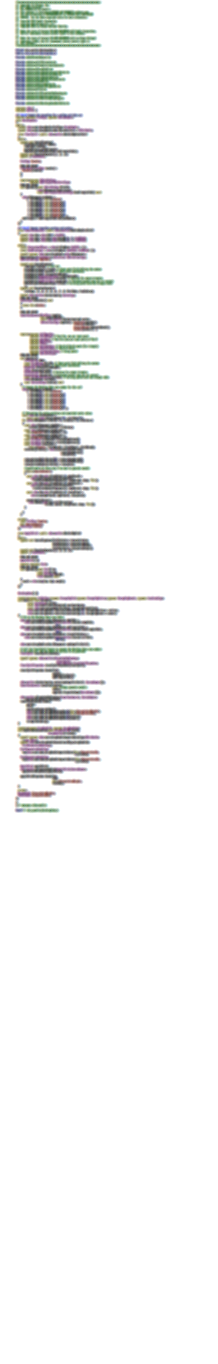
\includegraphics[width=.75in]{images/MCCompareVTKm}
  \end{tabular}
  \caption[Comparison of Marching Cubes implementations.]{Comparison of the
    Marching Cubes algorithm in VTK-m and two other implementations.
    Implementations in VTK-m are simpler, shorter, more general, and easier
    to maintain. (Lines of code (LOC) measurements come from cloc.}
  \label{fig:MCCompare}
\end{figure}

VTK-m simplifies the development of parallel scientific visualization
algorithms by providing a framework of supporting functionality that allows
developers to focus on visualization operations. Consider the listings in
Figure~\ref{fig:MCCompare} that compares the size of the implementations
for the Marching Cubes algorithm in VTK-m with the equivalent algorithms
implemented in the CUDA software development kit reference implementation
and the PISTON visualization library. Because VTK-m internally manages the
parallel distribution of work and data, the VTK-m implementation is shorter
and easier to maintain. Additionally, VTK-m provides data abstractions not
provided by the other libraries that make code written in VTK-m more
versatile.

\begin{didyouknow}
  VTK-m is written in C++ and makes extensive use of templates. The toolkit
  is implemented as a header library, meaning that all the code is
  implemented in header files (with extension \textfilename{.h}) and
  completely included in any code that uses it. This allows the compiler to
  inline and specialize code for better performance.
\end{didyouknow}

\section{How to Use This Guide}

This user's guide is organized into three parts to help guide novice to
advanced users and to provide a convenient reference.
Part~\ref{part:GettingStarted}, Getting Started, provides everything needed
to get up and running with VTK-m. In this part we learn the basics of
reading and writing data files, using filters to process data, and perform
basic rendering to view the results.

Part~\ref{part:Developing}, Developing with VTK-m, dives deeper into the
VTK-m library and provides all the information needed to customize VTK-m's
data structures and support multiple devices. Part~\ref{part:Developing}
also documents how to use VTK-m's framework to develop new or custom
visualization algorithms.

Part~\ref{part:Advanced}, Advanced Customization, exposes the inner
workings of VTK-m and allows you to design new algorithmic structures not
already available. \fix{This might be removed in the first version of the
  book.}

\section{Conventions Used in This Guide}

When documenting the VTK-m API, the following conventions are used.
\begin{itemize}
\item Filenames are printed in a \textfilename{sans serif font}.
\item C++ code is printed in a \textcode{monospace font}.
\item Macros and namespaces from VTK-m are printed in \textnamespace{red}.
\item Identifiers from VTK-m are printed in \textidentifier{blue}.
\item Signatures, described in Chapter~\ref{chap:Worklets}, and the
  tags used in them are printed in \textsignature{green}.
\end{itemize}

This guide provides actual code samples throughout its discussions to
demonstrate their use. These examples are all valid code that can be
compiled and used although it is often the case that code snippets are
provided. In such cases, the code must be placed in a larger context.

\begin{didyouknow}
  In this guide we periodically use these \textbf{Did you know?} boxes to
  provide additional information related to the topic at hand.
\end{didyouknow}

\begin{commonerrors}
  \textbf{Common Errors} blocks are used to highlight some of the common
  problems or complications you might encounter when dealing with the topic
  of discussion.
\end{commonerrors}


% -*- latex -*-

\chapter{Basic Provisions}
\label{chap:BasicProvisions}

This section describes the core facilities provided by VTK-m. These include
macros, types, and classes that define the environment in which code is
run, the core types of data stored, and template introspection. We also
start with a description of package structure used by VTK-m.


\section{General Approach}
\label{sec:GeneralApproach}

VTK-m is designed to provide a \keyterm{pervasive parallelism}
\index{pervasive parallelism} throughout all its visualization algorithms,
meaning that the algorithm is designed to operate with independent
concurrency at the finest possible level throughout. VTK-m provides this
pervasive parallelism by providing a programming construct called a
\keyterm{worklet}, \index{worklet} which operates on a very fine
granularity of data. The worklets are designed as serial components, and
VTK-m handles whatever layers of concurrency are necessary, thereby
removing the onus from the visualization algorithm developer. Worklet
operation is then wrapped into \keyterm{filters}, \index{filter} which
provide a simplified interface to end users.

A worklet is essentially a small functor \index{functor} or kernel
\index{kernel} designed to operate on a small element of data. (The name
``worklet'' means a small amount of work. We mean small in this sense to be
the amount of data, not necessarily the amount of instructions performed.)
The worklet is constrained to contain a serial and stateless function.
These constraints form three critical purposes. First, the constraints on
the worklets allow VTK-m to schedule worklet invocations on a great many
independent concurrent threads and thereby making the algorithm pervasively
parallel. Second, the constraints allow VTK-m to provide thread safety. By
controlling the memory access the toolkit can insure that no worklet will
have any memory collisions, false sharing, or other parallel programming
pitfalls. Third, the constraints encourage good programming practices. The
worklet model provides a natural approach to visualization algorithm design
that also has good general performance characteristics.

VTK-m allows developers to design algorithms that are run on massive
amounts of threads. However, VTK-m also allows developers to interface to
applications, define data, and invoke algorithms that they have written or
are provided otherwise. These two modes represent significantly different
operations on the data. The operating code of an algorithm in a worklet is
constrained to access only a small portion of data that is provided by the
framework. Conversely, code that is building the data structures needs to
manage the data in its entirety, but has little reason to perform
computations on any particular element.

Consequently, VTK-m is divided into two \keyterm{environments}
\index{environment} that handle each of these use cases. Each environment
has its own API, and direct interaction between the environments is
disallowed. The environments are as follows.

\begin{description}
\item[Execution Environment] \index{execution environment}
  \index{environment!execution} This is the environment in which the
  computational portion of algorithms are executed. The API for this
  environment provides work for one element with convenient access to
  information such as connectivity and neighborhood as needed by typical
  visualization algorithms. Code for the execution environment is designed
  to always execute on a very large number of threads.
\item[Control Environment] \index{control environment}
  \index{environment!control} This is the environment that is used to
  interface with applications, interface with I/O devices, and schedule
  parallel execution of the algorithms. The associated API is designed for
  users that want to use VTK-m to analyze their data using provided or
  supplied filters. Code for the control environment is designed to run on
  a single thread (or one single thread per process in an MPI job).
\end{description}

These dual programming environments are partially a convenience to isolate
the application from the execution of the worklets and are partially a
necessity to support GPU languages with host and device environments. The
control and execution environments are logically equivalent to the host and
device environments, respectively, in CUDA and other associated GPU
languages.

\begin{figure}[htb]
  \centering
  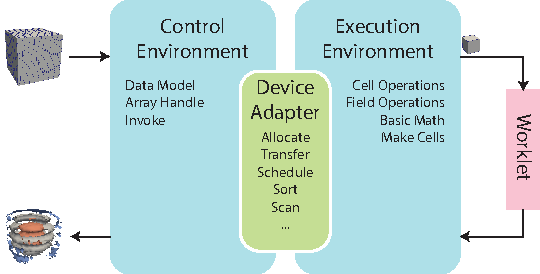
\includegraphics[width=4in]{images/VTKmEnvironments}
  \caption{Diagram of the VTK-m framework.}
  \label{fig:VTKmDiagram}
\end{figure}

Figure~\ref{fig:VTKmDiagram} displays the relationship between the control
and execution environment. The typical workflow when using VTK-m is that
first the control thread establishes a data set in the control environment
and then invokes a parallel operation on the data using a filter. From
there the data is logically divided into its constituent elements, which
are sent to independent invocations of a worklet. The worklet
invocations, being independent, are run on as many concurrent threads as
are supported by the device. On completion the results of the worklet
invocations are collected to a single data structure and a handle is
returned back to the control environment.

\begin{didyouknow}
  Are you only planning to use filters in VTK-m that already exist? If so,
  then everything you work with will be in the control environment. The
  execution environment is only used when implementing algorithms for
  filters.
\end{didyouknow}


\section{Package Structure}
\label{sec:PackageStructure}

\index{packages|(}

VTK-m is organized in a hierarchy of nested packages. VTK-m places
definitions in \keyterm{namespaces} \index{namespace} that correspond to
the package (with the exception that one package may specialize a template
defined in a different namespace).

The base package is named \vtkm{}. All classes within VTK-m are placed
either directly in the \vtkm{} package or in a package beneath it. This
helps prevent name collisions between VTK-m and any other library.

As described in Section~\ref{sec:GeneralApproach}, the VTK-m API is divided
into two distinct environments: \index{environment} the control environment
\index{control environment} \index{environment!control} and the execution
environment. \index{execution environment} \index{environment!execution}
The API for these two environments are located in the \vtkmcont{} and
\vtkmexec{} packages, respectively. Items located in the base \vtkm{}
namespace are available in both environments.

Although it is conventional to spell out names in identifiers (see the
coding conventions in Chapter~\ref{chap:CodingConventions}), there is an
exception to abbreviate control and execution to \textnamespace{cont}
and \textnamespace{exec}, respectively. This is because it is also part of
the coding convention to declare the entire namespace when using an
identifier that is part of the corresponding package. The shorter names
make the identifiers easier to read, faster to type, and more feasible to
pack lines in 80 column displays. These abbreviations are also used instead
of more common abbreviations (e.g. ctrl for control) because, as part of
actual English words, they are easier to type.

Further functionality in VTK-m is built on top of the base \vtkm{},
\vtkmcont{}, and \vtkmexec{} packages. Support classes for building
worklets, described in Chapter~\ref{chap:Worklets}, are contained in the
\vtkmworklet{} package. Other facilities in VTK-m are provided in their own
packages such as \vtkmio{}, \vtkmfilter{}, and \vtkmrendering{}. These
packages are described in Part~\ref{part:GettingStarted}.

VTK-m contains code that uses specialized compiler features, such as those
with CUDA, or libraries, such as Intel Threading Building Blocks, that will
not be available on all machines. Code for these features are encapsulated
in their own packages under the \vtkmcont{} namespace: \vtkmcontcuda{} and
\vtkmconttbb{}.

VTK-m contains OpenGL interoperability \index{OpenGL}
\index{interoperability} that allows data generated with VTK-m to be
efficiently transferred to OpenGL objects. This feature is encapsulated in
the \vtkmopengl{} package.

Figure~\ref{fig:Packages} provides a diagram of the VTK-m package hierarchy.

\begin{figure}[htb]
  \centering
  %% \begin{itemize}
  %% \item \vtkm{}
  %% \item \vtkmexec{}
  %% \item \vtkmcont{}
  %% \item \vtkmcontcuda{}
  %% \item \vtkmconttbb{}
  %% \item \vtkmio{}
  %% \item \vtkmioreader{}
  %% \item \vtkmiowriter{}
  %% \item \vtkmfilter{}
  %% \item \vtkmrendering{}
  %% \item \vtkmopengl{}
  %% \item \vtkmworklet{}
  %% %% \item \textnamespace{vtkm}
  %% %%   \begin{itemize}
  %% %%   \item \textnamespace{cont}
  %% %%   \item \textnamespace{exec}
  %% %%   \item \textnamespace{worklet}
  %% %%   \item \textnamespace{math}
  %% %%   \item \textnamespace{cuda}
  %% %%     \begin{itemize}
  %% %%     \item \textnamespace{cont}
  %% %%     \end{itemize}
  %% %%   \item \textnamespace{openmp}
  %% %%     \begin{itemize}
  %% %%     \item \textnamespace{cont}
  %% %%     \end{itemize}
  %% %%   \item \textnamespace{tbb}
  %% %%     \begin{itemize}
  %% %%     \item \textnamespace{cont}
  %% %%     \end{itemize}
  %% %%   \item \textnamespace{opengl}
  %% %%   \end{itemize}
  %% \end{itemize}
  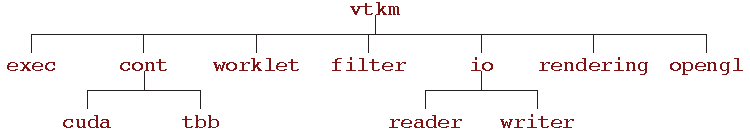
\includegraphics{images/PackageHierarchy}
  \caption{VTK-m package hierarchy.}
  \label{fig:Packages}
\end{figure}

By convention all classes will be defined in a file with the same name as
the class name (with a \textfilename{.h} extension) located in a directory
corresponding to the package name. For example, the \vtkmcont{ArrayHandle}
class is found in the \vtkmheader{vtkm/cont}{ArrayHandle.h} header. There
are, however, exceptions to this rule. Some smaller classes and types are
grouped together for convenience. These exceptions will be noted as
necessary.

Within each namespace there may also
be \textnamespace{internal}\indexnamespaceone{internal}
and \textnamespace{detail}\indexnamespaceone{detail}
sub-namespaces. The \textnamespace{internal} namespaces contain features
that are used internally and may change without
notice. The \textnamespace{detail} namespaces contain features that are
used by a particular class but must be declared outside of that
class. Users should generally ignore classes in these namespaces.

\index{packages|)}


\section{Function and Method Environment Modifiers}
\label{sec:FunctionAndMethodEnvironmentModifiers}

Any function or method defined by VTK-m must come with a modifier that determines in which environments the function may be run.
These modifiers are C macros that VTK-m uses to instruct the compiler for which architectures to compile each method.
Most user code outside of VTK-m need not use these macros with the important exception of any classes passed to VTK-m.
This occurs when defining new worklets, array storage, and device adapters.

VTK-m provides three modifier macros, \vtkmcontmodifier, \vtkmexecmodifier, and
\vtkmexeccontmodifier, which are used to declare functions and methods that
can run in the control environment, execution environment, and both
environments, respectively. These macros get defined by including just
about any VTK-m header file, but including \vtkmheader{vtkm}{Types.h} will
ensure they are defined. 

The modifier macro is placed after the template declaration, if there is one,
and before the return type for the function. Here is a simple example of a
function that will square a value. Since most types you would use this
function on have operators in both the control and execution environments,
the function is declared for both places.

\vtkmlisting{Usage of an environment modifier macro on a function.}{EnvironmentModifierMacro.cxx}

The primary function of the modifier macros is to inject compiler-specific
keywords that specify what architecture to compile code for. For example,
when compiling with CUDA\index{CUDA}, the control modifiers have
\textcode{\_\_host\_\_}\index{\_\_host\_\_} in them and execution modifiers
have \textcode{\_\_device\_\_}\index{\_\_device\_\_} in them.

There is one additional modifier macro that is not used for functions but
rather used when declaring a constant data object that is used in the
execution environment. This macro is named
\vtkmmacro{VTKM\_EXEC\_CONSTANT}\index{modifier!constant}\index{constant modifier}
and is used to declare a constant lookup table used when executing a
worklet. Its primary reason for existing is to add a
\textcode{\_\_constant\_\_} keyword when compiling with CUDA. This modifier
currently has no effect on any other compiler.

Finally, it is sometimes the case that a function declared as
\vtkmexeccontmodifier has to call a method declared as \vtkmexecmodifier or
\vtkmcontmodifier. Generally functions should not call other functions with
incompatible control/execution modifiers, but sometimes a generic
\vtkmexeccontmodifier function calls another function determined by the
template parameters, and the valid environments of this subfunction may be
inconsistent. For cases like this, you can use the
\vtkmmacro{VTKM\_SUPPRESS\_EXEC\_WARNINGS} to tell the compiler to ignore the
inconsistency when resolving the template. When applied to a templated
function or method, \vtkmmacro{VTKM\_SUPPRESS\_EXEC\_WARNINGS} is placed
before the \textcode{template} keyword. When applied to a non-templated
method in a templated class, \vtkmmacro{VTKM\_SUPPRESS\_EXEC\_WARNINGS} is
placed before the environment modifier macro.

\vtkmlisting{Suppressing warnings about functions from mixed environments.}{SuppressExecWarnings.cxx}


\section{Core Data Types}
\label{sec:CoreDataTypes}

Except in rare circumstances where precision is not a concern, VTK-m does
not directly use the core C types like \textcode{int}, \textcode{float},
and \textcode{double}. Instead, VTK-m provides its own core types, which
are declared in \vtkmheader{vtkm}{Types.h}.

\subsection{Single Number Types}

To ensure portability across different compilers and architectures, VTK-m
provides \textcode{typedef}s for the following basic types with explicit
precision: \vtkm{Float32}, \vtkm{Float64}, \vtkm{Int8}, \vtkm{Int16},
\vtkm{Int32}, \vtkm{Int64}, \vtkm{UInt8}, \vtkm{UInt16}, \vtkm{UInt32}, and
\vtkm{UInt64}. Under most circumstances when using VTK-m (and performing
visualization in general) the type of data is determined by the source of the
data or resolved through templates. In the case where a specific type of
data is required, these VTK-m--defined types should be preferred over basic
C types like \textcode{int} or \textcode{float}.

Many of the structures in VTK-m require indices to identify elements like
points and cells. All indices for arrays and other lists use the type
\vtkm{Id}. By default this type is a 32-bit wide integer but can be easily
changed by compile options. The CMake configuration option
\cmakevar{VTKM\_USE\_64BIT\_IDS} can be used to change \vtkm{Id} to be 64
bits wide. This configuration can be overridden by defining the C macro
\vtkmmacro{VTKM\_USE\_64BIT\_IDS} or \vtkmmacro{VTKM\_NO\_64BIT\_IDS} to
force \vtkm{Id} to be either 64 or 32 bits. These macros must be defined
before any VTK-m header files are included to take effect.

There is also a secondary index type named \vtkm{IdComponent} that is used
to index components of short vectors (discussed in
Section~\ref{sec:VectorTypes}). This type is an integer that might be a
shorter width than \vtkm{Id}.

There is also the rare circumstance in which an algorithm in VTK-m computes
data values for which there is no indication what the precision should
be. For these circumstances, the type \vtkm{FloatDefault} is provided. By
default this type is a 32-bit wide floating point number but can be easily
changed by compile options. The CMake configuration option
\cmakevar{VTKM\_USE\_DOUBLE\_PRECISION} can be used to change
\vtkm{FloatDefault} to be 64 bits wide. This configuration can be
overridden by defining the C macro \vtkmmacro{VTKM\_USE\_DOUBLE\_PRECISION}
or \vtkmmacro{VTKM\_NO\_DOUBLE\_PRECISION} to force \vtkm{FloatDefault} to
be either 64 or 32 bits. These macros must be defined before any VTK-m
header files are included to take
effect.

For convenience, you can include either
\vtkmheader{vtkm/internal}{ConfigureFor32.h} or
\vtkmheader{vtkm/internal}{ConfigureFor64.h} to force both \vtkm{Id} and
\vtkm{FloatDefault} to be 32 or 64 bits.

\subsection{Vector Types}
\label{sec:VectorTypes}

Visualization algorithms also often require operations on short vectors.
Arrays indexed in up to three dimensions are common. Data are often defined
in 2-space and 3-space, and transformations are typically done in
homogeneous coordinates of length 4. To simplify these types of operations,
VTK-m provides the \vtkm{Vec}\tparams{T,Size} templated type, which is
essentially a fixed length array of a given type.

The default constructor of \vtkm{Vec} objects leaves the values
uninitialized. All vectors have a constructor with one argument that is
used to initialize all components. All \vtkm{Vec} objects with a size of 4
or less is specialized to also have a constructor that allows you to set
the individual components. Likewise, there is a \vtkm{make\_Vec} function
that builds initialized vector types of up to 4 components. Once created,
you can use the bracket operator to get and set component values with the
same syntax as an array.

\vtkmlisting{Creating vector types.}{CreatingVectorTypes.cxx}

The types \vtkm{Id2} and \vtkm{Id3} are \textcode{typedef}s of
\vtkm{Vec}\tparams{\vtkm{Id},2} and \vtkm{Vec}\tparams{\vtkm{Id},2}. These
are used to index arrays of 2 and 3 dimensions, which is common.

Vectors longer than 4 are also supported, but independent component values must be set after construction.
The \vtkm{Vec} class contains a constant named \textidentifier{NUM\_COMPONENTS}\index{NUM\_COMPONENTS} to specify how many components are in the vector.
The class also has a \textcode{GetNumberOfComponents} method that also returns the number of components that are in the vector.

\vtkmlisting{A Longer Vector.}{LongerVector.cxx}

\vtkm{Vec} supports component-wise arithmetic using the operators
for plus (\textcode{+}), minus (\textcode{-}), multiply (\textcode{*}), and
divide (\textcode{/}). It also supports scalar to vector multiplication
with the multiply operator. The comparison operators equal (\textcode{==})
is true if every pair of corresponding components are true and not equal
(\textcode{!=}) is true otherwise. A special \vtkm{dot} function is
overloaded to provide a dot product for every type of vector.

\vtkmlisting{Vector operations.}{VectorOperations.cxx}

These operators, of course, only work if they are also defined for the
component type of the \vtkm{Vec}. For example, the multiply operator will
work fine on objects of type \vtkm{Vec}\tparams{char,3}, but the multiply
operator will not work on objects of type \vtkm{Vec}\tparams{std::string,3}
because you cannot multiply objects of type \textcode{std::string}.

In addition to generalizing vector operations and making arbitrarily long
vectors, \vtkm{Vec} can be repurposed for creating any sequence of
homogeneous objects. Here is a simple example of using \vtkm{Vec} to hold
the state of a polygon.

\vtkmlisting{Repurposing a \protect\vtkm{Vec}.}{EquilateralTriangle.cxx}

\index{Vec-like|(}

The \vtkm{Vec} class provides a convenient structure for holding and passing small vectors of data.
However, there are times when using \textidentifier{Vec} is inconvenient or inappropriate.
For example, the size of \vtkm{Vec} must be known at compile time, but there may be need for a vector whose size is unknown until compile time.
Also, the data populating a \vtkm{Vec} might come from a source that makes it inconvenient or less efficient to construct a \vtkm{Vec}.
For this reason, \VTKm also provides several \keyterm{\Veclike} objects that behave much like \vtkm{Vec} but are a different class.
These \Veclike objects have the same interface as \vtkm{Vec} except that the \textidentifier{NUM\_COMPONENTS} constant is not available on those that are sized at run time.
\Veclike objects also come with a \textcode{CopyInto} method that will take their contents and copy them into a standard \textidentifier{Vec} class.
(The standard \textidentifier{Vec} class also has a \textcode{CopyInto} method for consistency.)

The first \Veclike object is \vtkm{VecC}, which exposes a C-type array as a \textidentifier{Vec}.
The constructor for \vtkm{VecC} takes a C array and a size of that array.
There is also a constant version of \textidentifier{VecC} named \vtkm{VecCConst}, which takes a constant array and cannot be mutated.
The \vtkmheader{vtkm}{Types.h} header defines both \textidentifier{VecC} and \textidentifier{VecCConst} as well as multiple versions of \vtkm{make\_VecC} to easily convert a C array to either a \textidentifier{VecC} or \textidentifier{VecCConst}.

The following example demonstrates converting values from a constant table into a \vtkm{VecCConst} for further consumption.
The table and associated methods define how 8 points come together to form a hexahedron.

\vtkmlisting[ex:VecCConst]{Using \protect\vtkm{VecCConst} with a constant array.}{VecCExample.cxx}

\begin{commonerrors}
  The \vtkm{VecC} and \vtkm{VecCConst} classes only hold a pointer to a buffer that contains the data.
  They do not manage the memory holding the data.
  Thus, if the pointer given to \vtkm{VecC} or \vtkm{VecCConst} becomes invalid, then using the object becomes invalid.
  Make sure that the scope of the \vtkm{VecC} or \vtkm{VecCConst} does not outlive the scope of the data it points to.
\end{commonerrors}

The next \Veclike object is \vtkm{VecVariable}, which provides a \Veclike object that can be resized at run time to a maximum value.
Unlike \textidentifier{VecC}, \textidentifier{VecVariable} holds its own memory, which makes it a bit safer to use.
But also unlike \textidentifier{VecC}, you must define the maximum size of \textidentifier{VecVariable} at compile time.
Thus, \textidentifier{VecVariable} is really only appropriate to use when there is a predetermined limit to the vector size that is fairly small.

The following example uses a \vtkm{VecVariable} to store the trace of edges within a hexahedron.
This example uses the methods defined in Example~\ref{ex:VecCConst}.

\vtkmlisting{Using \protect\vtkm{VecVariable}.}{VecVariableExample.cxx}

\VTKm provides further examples of \Veclike objects as well.
For example, the \vtkm{VecFromPortal} and \vtkm{VecFromPortalPermute} objects allow you to treat a subsection of an arbitrarily large array as a \textidentifier{Vec}.
These objects work by attaching to array portals, which are described in Section~\ref{sec:ArrayPortals}.
Another example of a \Veclike object is \vtkm{VecRectilinearPointCoordinates}, which efficiently represents the point coordinates in an axis-aligned hexahedron.
Such shapes are common in structured grids.
These and other data sets are described in Chapter~\ref{chap:DataSets}.

\index{Vec-like|)}


\subsection{Pair}
\label{sec:Pair}

VTK-m defines a \vtkm{Pair}\tparams{T1,T2} templated object that
behaves just like \textcode{std:\colonhyp{}pair} from the standard template
library. The difference is that \vtkm{Pair} will work in both the execution
and control environment, whereas the STL \textcode{std::pair} does not
always work in the execution environment.

The VTK-m version of \vtkm{Pair} supports the same types, fields, and
operations as the STL version. VTK-m also provides a \vtkm{make\_Pair}
function for convenience.

\subsection{Range}
\label{sec:Range}

VTK-m provides a convenience structure named \vtkm{Range} to help manage a
range of values. The \textidentifier{Range} \textcode{struct} contains two
data members, \textcode{Min} and \textcode{Max}, which represent the ends
of the range of numbers. \textcode{Min} and \textcode{Max} are both of type
\vtkm{Float64}. \textcode{Min} and \textcode{Max} can be directly accessed,
but \textidentifier{Range} also comes with the following helper functions
to make it easier to build and use ranges. Note that all of these functions
treat the minimum and maximum value as inclusive to the range.

\begin{description}
\item[\textcode{IsNonEmpty}] Returns true if the range covers at least one
  value.
\item[\textcode{Contains}] Takes a single number and returns true if that
  number is contained within the range.
\item[\textcode{Length}] Returns the distance between \textcode{Min} and
  \textcode{Max}. Empty ranges return a length of 0. Note that if the range
  is non-empty and the length is 0, then \textcode{Min} and \text{Max} must
  be equal, and the range contains exactly one number.
\item[\textcode{Center}] Returns the number equidistant to \textcode{Min}
  and \textcode{Max}. If the range is empty, NaN is returned.
\item[\textcode{Include}] Takes either a single number or another range and
  modifies this range to include the given number or range. If necessary,
  the range is grown just enough to encompass the given argument. If the
  argument is already in the range, nothing changes.
\item[\textcode{Union}] A nondestructive version of \textcode{Include},
  which builds a new \textidentifier{Range} that is the union of this range
  and the argument. The \textcode{+} operator is also overloaded to compute
  the union.
\end{description}

The following example demonstrates the operation of \vtkm{Range}.

\vtkmlisting{Using \protect\vtkm{Range}.}{UsingRange.cxx}

\subsection{Bounds}
\label{sec:Bounds}

VTK-m provides a convenience structure named \vtkm{Bounds} to help manage
an axis-aligned region in 3D space. Among other things, this structure is
often useful for representing a bounding box for geometry. The
\textidentifier{Bounds} \textcode{struct} contains three data members,
\textcode{X}, \textcode{Y}, and \textcode{Z}, which represent the range of
the bounds along each respective axis. All three of these members are of
type \vtkm{Range}, which is discussed previously in
Section~\ref{sec:Range}. \textcode{X}, \textcode{Y}, and \textcode{Z} can
be directly accessed, but \textidentifier{Bounds} also comes with the
following helper functions to make it easier to build and use ranges.

\begin{description}
\item[\textcode{IsNonEmpty}] Returns true if the bounds cover at least one
  value.
\item[\textcode{Contains}] Takes a \vtkm{Vec} of size 3 and returns true if
  those point coordinates are contained within the range.
\item[\textcode{Center}] Returns the point at the center of the range as a
  \vtkm{Vec}\textcode{<}\vtkm{Float64}\textcode{,3>}.
\item[\textcode{Include}] Takes either a \vtkm{Vec} of size 3 or another
  bounds and modifies this bounds to include the given point or bounds. If
  necessary, the bounds are grown just enough to encompass the given
  argument. If the argument is already in the bounds, nothing changes.
\item[\textcode{Union}] A nondestructive version of \textcode{Include},
  which builds a new \textidentifier{Bounds} that is the union of this
  bounds and the argument. The \textcode{+} operator is also overloaded to
  compute the union.
\end{description}

The following example demonstrates the operation of \vtkm{Bounds}.

\vtkmlisting{Using \protect\vtkm{Bounds}.}{UsingBounds.cxx}


\section{Traits}
\label{sec:Traits}

\index{traits|(}

When using templated types, it is often necessary to get information about
the type or specialize code based on general properties of the type. VTK-m
uses traits classes to publish and retrieve information about types. A
traits class is simply a templated structure that provides typedefs for
tag\index{tag} structures, empty types used for identification. The traits
classes might also contain constant numbers and helpful static
functions. See {\it Effective C++ Third Edition} by Scott Mayers for a
description of traits classes and their uses.

\subsection{Type Traits}

\index{traits!type|(}
\index{type traits|(}

The \vtkm{TypeTraits}\tparams{T} templated class provides basic information
about a core type. These type traits are available for all the basic C++
types as well as the core VTK-m types described in
Section~\ref{sec:CoreDataTypes}. \vtkm{TypeTraits} contains the following
elements.

\index{tag!type traits|(}

\begin{description}
\item[\textidentifier{NumericTag}] \index{NumericTag} \index{tag!numeric}
  This type is set to either \vtkm{TypeTraitsRealTag} or
  \vtkm{TypeTraitsIntegerTag} to signal that the type represents either
  floating point numbers or integers.
\item[\textidentifier{DimensionalityTag}] \index{DimensionalityTag}
  \index{tag!dimensionality} This type is set to either
  \vtkm{TypeTraitsScalarTag} or \vtkm{TypeTraitsVectorTag} to signal that
  the type represents either a single scalar value or a tuple of values.
\item[\textidentifier{ZeroInitialization}] \index{ZeroInitialization}
  A static member function that takes no arguments and returns 0 (or the closest equivalent to it) cast to the type.
\end{description}

The definition of \vtkm{TypeTraits} for \vtkm{Float32} could like something
like this.
\vtkmlisting{Definition of \protect \vtkm{TypeTraits}\tparams{\protect \vtkm{Float32}}.}{TypeTraitsImpl.cxx}

Here is a simple example of using \vtkm{TypeTraits} to implement a generic
function that behaves like the remainder operator (\textcode{\%}) for all
types including floating points and vectors.

\vtkmlisting[ex:TypeTraits]{Using \textidentifier{TypeTraits} for a generic remainder.}{TypeTraits.cxx}

\index{tag!type traits|)}

\index{type traits|)}
\index{traits!type|)}


\subsection{Vector Traits}
\label{sec:VectorTraits}

\index{traits!vector|(}
\index{vector traits|(}

The templated \vtkm{Vec} class contains several items for introspection (such as the component type and its size).
However, there are other types behave similarly to \textidentifier{Vec} objects but have different ways to perform this introspection.
\index{Vec-like} For example, \VTKm contains \Veclike objects that essentially behave the same but might have different features such as a variable number of components.
Also, there may be reason to interchangeably use basic scalar values, like an integer or floating point number, with vectors.

To provide a consistent interface to access these multiple types that represents vectors, the \vtkm{VecTraits}\tparams{T} templated class provides information and accessors to vector types.
It contains the following elements.

\index{tag!vector traits|(}

\begin{description}
\item[\textidentifier{ComponentType}]
  \index{ComponentType}
  This type is set to the type for each component in the vector.
  For example, a \vtkm{Id3} has \textidentifier{ComponentType} defined as \vtkm{Id}.
\item[\textidentifier{IsSizeStatic}]
  \index{IsSizeStatic} \index{tag!static vector size} \index{tag!variable vector size}
  This type is set to either \vtkm{VecTraitsTagSizeStatic} if the vector has a static number of components that can be determined at compile time or set to \vtkm{VecTraitsTagSizeVariable} if the size of the vector is determined at run time.
  If \textidentifier{IsSizeStatic} is set to \textidentifier{VecTraitsTagSizeVariable}, then \textidentifier{VecTraits} will be missing some information that cannot be determined at compile time.
\item[\textidentifier{HasMultipleComponents}]
  \index{HasMultipleComponents} \index{tag!single component} \index{tag!multiple components}
  This type is set to either \vtkm{VecTraitsTagSingleComponent} if the vector length is size 1 or \vtkm{VecTraitsTagMultipleComponents} otherwise.
  This tag can be useful for creating specialized functions when a vector is really just a scalar.
  If the vector type is of variable size (that is, \textidentifier{IsSizeStatic} is \textidentifier{VecTraitsTagSizeVariable}), then \textidentifier{HasMultipleComponents} might be \textidentifier{VecTraitsTagMultipleComponents} even when at run time there is only one component.
\item[\textidentifier{NUM\_COMPONENTS}] \index{NUM\_COMPONENTS}
  An integer specifying how many components are contained in the vector.
  \textidentifier{NUM\_COMPONENTS} is not available for vector types of variable size (that is, \textidentifier{IsSizeStatic} is \textidentifier{VecTraitsTagSizeVariable}).
\item[\textcode{GetNumberOfComponents}] \index{GetNumberOfComponents}
  A static method that takes an instance of a vector and returns the number of components the vector contains.
  The result of \textcode{GetNumberOfComponents} is the same value of \textidentifier{NUM\_COMPONENTS} for vector types that have a static size (that is, \textidentifier{IsSizeStatic} is \textidentifier{VecTraitsTagSizeStatic}).
  But unlike \textidentifier{NUM\_COMPONENTS}, \textcode{GetNumberOfComponents} works for vectors of any type.
\item[\textcode{GetComponent}] \index{GetComponent}
  A static method that takes a vector and returns a particular component.
\item[\textcode{SetComponent}] \index{SetComponent}
  A static method that takes a vector and sets a particular component to a given value.
\item[\textcode{CopyInto}] \index{CopyInto}
  A static method that copies the components of a vector to a \vtkm{Vec}.
\end{description}

The definition of \vtkm{VecTraits} for \vtkm{Id3} could look something like
this.
\vtkmlisting{Definition of \protect \vtkm{VecTraits}\tparams{\protect \vtkm{Id3}}.}{VecTraitsImpl.cxx}

\index{tag!vector traits|)}

The real power of vector traits is that they simplify creating generic
operations on any type that can look like a vector. This includes
operations on scalar values as if they were vectors of size one. The
following code uses vector traits to simplify the implementation of less
functors\index{less} that define an ordering that can be used for sorting
and other operations.

\vtkmlisting{Using \textidentifier{VecTraits} for less functors.}{VecTraits.cxx}

\index{vector traits|)}
\index{traits!vector|)}

\index{traits|)}


\section{List Tags}
\label{sec:ListTags}

\index{tag!lists|(}
\index{lists|(}

\index{template metaprogramming}
\index{metaprogramming}
VTK-m internally uses template metaprogramming, which utilizes C++
templates to run source-generating programs, to customize code to various
data and compute platforms. One basic structure often uses with template
metaprogramming is a list of class names (also sometimes called a tuple or
vector, although both of those names have different meanings in VTK-m).

Many VTK-m users only need predefined lists, such as the type lists
specified in Section~\ref{sec:TypeLists}. Those users can skip most of the
details of this section. However, it is sometimes useful to modify lists,
create new lists, or operate on lists, and these usages are documented
here.

VTK-m uses a tag-based mechanism for defining lists, which differs
significantly from lists in many other template metaprogramming libraries
such as with \textcode{boost:\colonhyp{}mpl:\colonhyp{}vector} or
\textcode{boost:\colonhyp{}vector}. Rather than enumerating all list
entries as template arguments, the list is referenced by a single tag class
with a descriptive name. The intention is to make fully resolved types
shorter and more readable. (Anyone experienced with template programming
knows how insanely long and unreadable types can get in compiler errors and
warnings.)

\subsection{Building List Tags}
\label{sec:BuildingListTags}

List tags are constructed in VTK-m by defining a \textcode{struct} that
publicly inherits from another list tags. The base list tags are defined in
the \vtkmheader{vtkm}{ListTag.h} header.

The most basic list is defined with \vtkm{ListTagEmpty}. This tag
represents an empty list.

\vtkm{ListTagBase}\tparams{T, ...} represents a list of the types given as
template parameters. \vtkm{ListTagBase} supports a variable number of
parameters with the maximum specified by \vtkmmacro{VTKM\_MAX\_BASE\_LIST}.

Finally, lists can be combined together with
\vtkm{ListTagJoin}\tparams{ListTag1,ListTag2}, which concatinates two lists
together.

The following example demonstrates how to build list tags using these base
lists classes. Note first that all the list tags are defined as
\textcode{struct} rather than \textcode{class}. Although these are roughly
synonymous in C++, \textcode{struct} inheritance is by default public, and
public inheritance is important for the list tags to work. Note second that
these tags are created by inheritance rather than using
\textcode{typedef}. Although \textcode{typedef} will work, it will lead to
much uglier type names defined by the compiler.

\vtkmlisting{Creating list tags.}{BaseListTags.cxx}

\subsection{Type Lists}
\label{sec:TypeLists}

\index{type lists|(}
\index{lists!types|(}
\index{tag!type lists|(}

One of the major use cases for template metaprogramming lists in VTK-m is
to identify a set of potential data types for arrays. The
\vtkmheader{vtkm}{TypeListTag.h} header contains predefined lists for known
VTK-m types. Although technically all these lists are of C++ types, the
types we refer to here are those data types stored in data arrays. The
following lists are provided.

\begin{description}
\item[\vtkm{TypeListTagId}] Contains the single item \vtkm{Id}.
\item[\vtkm{TypeListTagId2}] Contains the single item \vtkm{Id2}.
\item[\vtkm{TypeListTagId3}] Contains the single item \vtkm{Id3}.
\item[\vtkm{TypeListTagIndex}] A list of all types used to index
  arrays. Contains \vtkm{Id}, \vtkm{Id2}, and \vtkm{Id3}.
\item[\vtkm{TypeListTagFieldScalar}] A list containing types used for
  scalar fields. Specifically, it contains floating point numbers of
  different widths (i.e. \vtkm{Float32} and \vtkm{Float64}).
\item[\vtkm{TypeListTagFieldVec2}] A list containing types for values of
  fields with 2 dimensional vectors. All these vectors use floating point
  numbers.
\item[\vtkm{TypeListTagFieldVec3}] A list containing types for values of
  fields with 3 dimensional vectors. All these vectors use floating point
  numbers.
\item[\vtkm{TypeListTagFieldVec3}] A list containing types for values of
  fields with 3 dimensional vectors. All these vectors use floating point
  numbers.
\item[\vtkm{TypeListTagField}] A list containing all the types generally
  used for fields. It is the combination of \vtkm{TypeListTagFieldScalar},
  \vtkm{TypeListTagFieldVec2}, \vtkm{TypeListTagFieldVec3}, and
  \vtkm{TypeListTagFieldVec4}.
\item[\vtkm{TypeListTagScalarAll}] A list of all scalar types. It contains
  signed and unsigned integers of widths from 8 to 64 bits. It also
  contains floats of 32 and 64 bit widths.
\item[\vtkm{TypeListTagVecCommon}] A list of the most common vector
  types. It contains all \vtkm{Vec} class of size 2 through 4 containing
  components of unsigned bytes, signed 32-bit integers, signed 64-bit
  integers, 32-bit floats, or 64-bit floats.
\item[\vtkm{TypeListTagVecAll}] A list of all \vtkm{Vec} classes with
  standard integers or floating points as components and lengths between 2
  and 4.
\item[\vtkm{TypeListTagAll}] A list of all types included in
  \vtkmheader{vtkm}{Types.h} with \vtkm{Vec}s with up to 4 components.
\item[\vtkm{TypeListTagCommon}] A list containing only the most used types
  in visualization. This includes signed integers and floats that are 32 or
  64 bit. It also includes 3 dimensional vectors of floats. This is the
  default list used when resolving the type in dynamic arrays (described in
  Chapter~\ref{chap:DynamicArrayHandle}).
\end{description}

If these lists are not sufficient, it is possible to build new type lists
using the existing type lists and the list bases from
Section~\ref{sec:BuildingListTags} as demonstrated in the following
example.

\vtkmlisting[ex:CustomTypeLists]{Defining new type lists.}{CustomTypeLists.cxx}

The \vtkmheader{vtkm}{TypeListTag.h} header also defines a macro named
\vtkmmacro{VTKM\_DEFAULT\_TYPE\_LIST\_TAG} that defines a default list of
types to use in classes like \vtkmcont{DynamicArrayHandle}
(Chapter~\ref{chap:DynamicArrayHandle}). This list can be overridden by
defining the \vtkmmacro{VTKM\_DEFAULT\_TYPE\_LIST\_TAG} macro \emph{before}
any VTK-m headers are included. If included after a VTK-m header, the list
is not likely to take effect. Do not ignore compiler warnings about the
macro being redefined, which you will not get if defined
correctly. Example~\ref{ex:CustomTypeLists} also contains an example of
overriding the \vtkmmacro{VTKM\_DEFAULT\_TYPE\_LIST\_TAG} macro.

\index{tag!type lists|)}
\index{lists!types|)}
\index{type lists|)}

\subsection{Operating on Lists}
\label{sec:OperatingOnLists}

VTK-m template metaprogramming lists are typically just passed to VTK-m
methods that internally operate on the lists. Although not typically used
outside of the VTK-m library, these operations are also available.

The \vtkmheader{vtkm}{ListTag.h} header comes with a \vtkm{ListForEach}
function that takes a functor object and a list tag. It then calls the
functor object with the default object of each type in the list. This is
most typically used with C++ run-time type information to convert a
run-time polymorphic object to a statically typed (and possibly inlined)
call.

The following example shows a rudimentary version of coverting a
dynamically-typed array to a statically-typed array similar to what is done
in VTK-m classes like \vtkmcont{DynamicArrayHandle} (which is documented in
Chapter~\ref{chap:DynamicArrayHandle}).

\vtkmlisting{Converting dynamic types to static types with \textidentifier{ListForEach}.}{ListForEach.cxx}

\index{lists|)}
\index{tag!lists|)}


\section{Error Handling}
\label{sec:ErrorHandlingControl}

\index{errors|(}

\index{errors!control environment|(}

VTK-m uses exceptions to report errors. All exceptions thrown by VTK-m will
be a subclass of \vtkmcont{Error}. For simple error reporting, it is
possible to simply catch a \vtkmcont{Error} and report the error message
string reported by the \textcode{GetMessage} method.

\vtkmlisting{Simple error reporting.}{CatchingErrors.cxx}

There are several subclasses to \vtkmcont{Error}. The specific subclass
gives an indication of the type of error that occured when the exception
was thrown. Catching one of these subclasses may help a program better
recover from errors.
\begin{description}
\item[\vtkmcont{ErrorBadAllocation}] Thrown when there is a problem
  accessing or manipulating memory. Often this is thrown when an allocation
  fails because there is insufficient memory, but other memory access
  errors can cause this to be thrown as well.
\item[\vtkmcont{ErrorBadType}] Thrown when VTK-m attempts to perform
  an operation on an object that is of an incompatible type.
\item[\vtkmcont{ErrorBadValue}] Thrown when a VTK-m function or
  method encounters an invalid value that inhibits progress.
\item[\vtkmcont{ErrorExecution}] \index{errors!execution environment} Throw
  when an error is signaled in the execution environment for example when a
  worklet is being executed.
\item[\vtkmcont{ErrorInternal}] Thrown when VTK-m detects an
  internal state that should never be reached. This error usually indicates
  a bug in VTK-m or, at best, VTK-m failed to detect an invalid input it
  should have.
\item[\vtkmio{ErrorIO}] Thrown by a reader or writer when a file error is
  encountered.
\end{description}

\index{errors!control environment|)}

\index{assert|(}
\index{errors!assert|(}

In addition to the aforementioned error signaling, the
\vtkmheader{vtkm}{Assert.h} header file defines a macro named
\vtkmmacro{VTKM\_ASSERT}. This macro behaves the same as the POSIX
\textmacro{assert} macro. It takes a single argument that is a condition
that is expected to be true. If it is not true, the program is halted and a
message is printed. Asserts are useful debugging tools to ensure that
software is behaving and being used as expected.

\vtkmlisting{Using \protect\vtkmmacro{VTKM\_ASSERT}.}{Assert.cxx}

\begin{didyouknow}
  Like the POSIX \textmacro{assert}, if the \vtkmmacro{NDEBUG} macro is
  defined, then \vtkmmacro{VTKM\_ASSERT} will become an empty expression.
  Typically \vtkmmacro{NDEBUG} is defined with a compiler flag (like
  \textcode{-DNDEBUG}) for release builds to better optimize the code.
  CMake will automatically add this flag for release builds.
\end{didyouknow}

\begin{commonerrors}
  A helpful warning provided by many compilers alerts you of unused
  variables. (This warning is commonly enabled on VTK-m regression test
  nightly builds.) If a function argument is used only in a
  \vtkmmacro{VTKM\_ASSERT}, then it will be required for debug builds and
  be unused in release builds. To get around this problem, add a statement
  to the function of the form \textcode{(void)\textit{variableName};}. This
  statement will have no effect on the code generated but will suppress the
  warning for release builds.
\end{commonerrors}

\index{assert!static|(}
\index{static assert|(}

Because \VTKm makes heavy use of C++ templates, it is possible that these templates could be used with inappropriate types in the arguments.
Using an unexpected type in a template can lead to very confusing errors, so it is better to catch such problems as early as possible.
The \vtkmmacro{VTKM\_STATIC\_ASSERT} macro, defined in \vtkmheader{vtkm}{StaticAssert.h} makes this possible.
This macro takes a constant expression that can be evaluated at compile time and verifies that the result is true.

In the following example, \vtkmmacro{VTKM\_STATIC\_ASSERT} and its sister macro \vtkmmacro{VTKM\_STATIC\_ASSERT\_MSG}, which allows you to give a descriptive message for the failure, are used to implement checks on a templated function that is designed to work on any scalar type that is represented by 32 or more bits.

\vtkmlisting[ex:StaticAssert]{Using \protect\vtkmmacro{VTKM\_STATIC\_ASSERT}.}{StaticAssert.cxx}

\begin{didyouknow}
  \index{is\_same}
  In addition to the several trait template classes provided by \VTKm to introspect C++ types, the C++ standard \textfilename{type\_traits} header file contains several helpful templates for general queries on types.
  Example~\ref{ex:StaticAssert} demonstrates the use of one such template: \textcode{std::is\_same}.
\end{didyouknow}

\begin{commonerrors}
  \index{true\_type} \index{false\_type} \index{type\_traits}
  Many templates used to introspect types resolve to the tags \textcode{std::true\_type} and \textcode{std::false\_type} rather than the constant values \textcode{true} and \textcode{false} that \vtkmmacro{VTKM\_STATIC\_ASSERT} expects.
  The \textcode{std::true\_type} and \textcode{std::false\_type} tags can be converted to the Boolean literal by adding \textcode{::value} to the end of them.
  Failing to do so will cause \vtkmmacro{VTKM\_STATIC\_ASSERT} to behave incorrectly.
  Example~\ref{ex:StaticAssert} demonstrates getting the Boolean literal from the result of \textcode{std::is\_same}.
\end{commonerrors}

\index{static assert|)}
\index{assert!static|)}

\index{errors!assert|)}
\index{assert|)}

\index{errors|)}


\section{\VTKm Version}
\label{sec:Version}

\index{version|(}

As the \VTKm code evolves, changes to the interface and behavior will inevitably happen.
Consequently, code that links into \VTKm might need a specific version of \VTKm or changes its behavior based on what version of \VTKm it is using.
To facilitate this, \VTKm software is managed with a versioning system and advertises its version in multiple ways.
As with many software products, \VTKm has three version numbers: major, minor, and patch.
The major version represents significant changes in the \VTKm implementation and interface.
Changes in the major version include backward incompatible changes.
The minor version represents added functionality.
Generally, changes in the minor version to not introduce changes to the API (although the early 1.X versions of \VTKm violate this).
The patch version represents fixes provided after a release occurs.
Patch versions represent minimal change and do not add features.

\index{version!CMake|(}
\index{CMake|(}
\index{CMake!version|(}
\index{CMake!VTK-m package!version|(}
\index{VTK-m CMake package!version|(}

If you are writing a software package that is managed by CMake and load \VTKm with the \textcode{find\_package} command as described in Section~\ref{sec:LinkingToVTKm}, then you can query the \VTKm version directly in the CMake configuration.
When you load \VTKm with \textcode{find\_package}, CMake sets the variables \cmakevar{VTKm\_VERSION\_MAJOR}, \cmakevar{VTKm\_VERSION\_MINOR}, and \cmakevar{VTKm\_VERSION\_PATCH} to the major, minor, and patch versions, respectively.
Additionally, \cmakevar{VTKm\_VERSION} is set to the ``major.minor'' version number and \cmakevar{VTKm\_VERSION\_FULL} is set to the ``major.minor.patch'' version number.
If the current version of \VTKm is actually a development version that is in between releases of \VTKm, then and abbreviated SHA of the git commit is also included as part of \cmakevar{VTKm\_VERSION\_FULL}.

\begin{didyouknow}
  If you have a specific version of \VTKm required for your software, you can also use the version option to the \textcode{find\_package} CMake command.
  The \textcode{find\_package} command takes an optional version argument that causes the command to fail if the wrong version of the package is found.
\end{didyouknow}

\index{VTK-m CMake package!version|)}
\index{CMake!VTK-m package!version|)}
\index{CMake!version|)}
\index{CMake|)}
\index{version!CMake|)}

\index{version!macro|(}

It is also possible to query the \VTKm version directly in your code through preprocessor macros.
The \vtkmheader{vtkm}{Version.h} header file defines the following preprocessor macros to identify the \VTKm version.
\vtkmmacro{VTKM\_VERSION\_MAJOR}, \vtkmmacro{VTKM\_VERSION\_MINOR}, and \vtkmmacro{VTKM\_VERSION\_PATCH} are set to integer numbers representing the major, minor, and patch versions, respectively.
Additionally, \vtkmmacro{VTKM\_VERSION} is set to the ``major.minor'' version number as a string and \vtkmmacro{VTKM\_VERSION\_FULL} is set to the ``major.minor.patch'' version number (also as a string).
If the current version of \VTKm is actually a development version that is in between releases of \VTKm, then and abbreviated SHA of the git commit is also included as part of \vtkmmacro{VTKM\_VERSION\_FULL}.

\begin{commonerrors}
  Note that the CMake variables all begin with \textcode{VTKm\_} (lowercase ``m'') whereas the preprocessor macros begin with \textcode{VTKM\_} (all uppercase).
  This follows the respective conventions of CMake variables and preprocessor macros.
\end{commonerrors}

Note that \vtkmheader{vtkm}{Version.h} does not include any other \VTKm header files.
This gives your code a chance to load, query, and react to the \VTKm version before loading any \VTKm code proper.

\index{version!macro|)}

\index{version|)}


\chapter{Provided Worklets}
\label{chap:ProvidedWorklets}

\fix{Write this once some worklets are provided. I expect before this we
  will have a chapter on provided filters. In fact, that probably means
  this chapter should move after the chapters on control and execution
  environments.}

% -*- latex -*-

\chapter{Control Environment}
\label{chap:ControlEnvironment}

\index{control~environment|(}
\index{environment!control|(}

The control environment is where code interfaces with applications and I/O
devices. The associated API is designed for users that want to use VTK-m to
analyze their data using provided or supplied worklets. Code for the
control environment is designed to run on a single thread (or one single
thread per process in an MPI job).

Most users of VTK-m will have some interaction with the control
environment, for you cannot define data structures or execute any
algorithms without it.

\section{Array Handle}
\label{sec:ArrayHandle}

\index{array~handle|(}

\subsection{Basic Storage}

\index{array~handle!storage|(}
\index{storage|(}

As previously discussed, \vtkmcont{ArrayHandle} takes two template arguments.
\begin{vtkmexample}{Declaration of the \protect\vtkmcont{ArrayHandle} templated class (again).}
template<
    typename T,
    typename StorageTag = VTKM_DEFAULT_STORAGE_TAG>
class ArrayHandle;
\end{vtkmexample}
The first argument is the only one required and has been demonstrated
multiple times before. The second (optional) argument specifies something
called a storage, which provides the interface between the generic
\vtkmcont{ArrayHandle} class and a specific storage mechanism in the
control environment.

In this and the following sections we describe this storage mechanism.  A
default storage is specified in much the same way as a default device
adapter is defined. It is done by setting the \vtkmmacro{VTKM\_STORAGE}
macro. This macro must be set before including any VTK-m header
files. Currently the only practical storage provided by VTK-m is the basic
storage, which simply allocates a continuous section of memory of the given
base type. This storage can be explicitly specified by setting
\vtkmmacro{VTKM\_STORAGE} to \vtkmmacro{VTKM\_STORAGE\_BASIC} although the
basic storage will also be used as the default if no other storage is
specified (which is typical).

The default storage can always be overridden by specifying an array
storage tag. The tag for the basic storage is located in the
\vtkmheader{vtkm/cont}{StorageBasic.h} header file and is named
\vtkmcont{StorageTagBasic}. Here is an example of specifying
the storage type when declaring an array handle.

\vtkmlisting{Specifying the storage type for an \textidentifier{ArrayHandle.}}{ArrayHandleStorageParameter.cxx}

VTK-m also defines a macro named \vtkmmacro{VTKM\_DEFAULT\_STORAGE\_TAG}
that can be used in place of an explicit storage tag to use the
default tag. This macro is used to create new templates that have template
parameters for storage that can use the default.

\subsection{Adapting Data Structures}
\label{sec:ArrayHandle:Adapting}

\index{array~handle!adapting|(}
\index{storage!adapting|(}

The intention of the storage parameter for \vtkmcont{ArrayHandle} is to
implement the strategy design pattern to enable VTK-m to interface directly
with the data of any third party code source. VTK-m is designed to work
with data originating in other libraries or applications. By creating a new
type of storage, VTK-m can be entirely adapted to new kinds of data
structures.

In this section we demonstrate the steps required to adapt the array handle
to a data structure provided by a third party. For the purposes of the
example, let us say that some fictitious library named ``foo'' has a simple
structure named \textcode{FooFields} that holds the field values for a
particular part of a mesh, and then maintain the field values for all
locations in a mesh in a \textcode{std::deque} object.

\vtkmlisting{Fictitious field storage used in custom array storage examples.}{FictitiousFieldStorage.cxx}

VTK-m expects separate arrays for each of the fields rather than a single
array containing a structure holding all of the fields. However, rather
than copy each field to its own array, we can create a storage for each
field that points directly to the data in a \textcode{FooFieldsDeque}
object.

The first step in creating an adapter storage is to create a control
environment array portal to the data. This is described in more detail in
Section~\ref{sec:ArrayPortals} and is generally straightforward for simple
containers like this. Here is an example implementation for our
\textcode{FooFieldsDeque} container.

\vtkmlisting[ex:ArrayPortalAdapter]{Array portal to adapt a third-party container to VTK-m.}{ArrayPortalAdapter.cxx}

The next step in creating an adapter storage is to define a tag for the
adapter. We shall call ours
\textcode{StorageTagFooPressure}. Then, we need to create a
specialization of the templated \vtkmcontinternal{Storage}
class. The \textidentifier{ArrayHandle} will instantiate an object using
the array container tag we give it, and we define our own specialization so
that it runs our interface into the code.

\vtkmcontinternal{Storage} has two template arguments: the
base type of the array and the storage tag.

\vtkmlisting{Prototype for \protect\vtkmcontinternal{Storage}.}{StoragePrototype.cxx}

The \vtkmcontinternal{Storage} must define the following items.
\begin{description}
\item[\textcode{ValueType}] A \textcode{typedef} of the type for each item
  in the array. This is the same type as the first template argument.
\item[\textcode{PortalType}] The type of an array portal that can be used
  to access the underlying data. This array portal needs to work only in
  the control environment.
\item[\textcode{PortalConstType}] A read-only (const) version of
  \textcode{PortalType}.
\item[\textcode{GetPortal}] A method that returns an array portal of type
  \textcode{PortalType} that can be used to access the data manged in this
  storage.
\item[\textcode{GetPortalConst}] Same as \textcode{GetPortal} except it
  returns a read-only (const) array portal.
\item[\textcode{GetNumberOfValues}] A method that returns the number of
  values the storage is currently allocated for.
\item[\textcode{Allocate}] A method that allocates the array to a given
  size. An values stored in the previous allocation may be destroyed.
\item[\textcode{Shrink}] A method like \textcode{Allocate} with two
  differences. First, the size of the allocation must be smaller than the
  existing allocation when the method is called. Second, any values
  currently stored in the array will be valid after the array is
  resized. This constrained form of allocation allows the array to be
  resized and values valid without ever having to copy data.
\item[\textcode{ReleaseResources}] A method that instructs the storage to
  free all of its memory.
\end{description}

The following provides an example implementation of our adapter to a
\textcode{FooFieldsDeque}. It relies on the
\textcode{ArrayPortalFooPressure} provided in
Example~\ref{ex:ArrayPortalAdapter}.

\vtkmlisting{Storage to adapt a third-party container to VTK-m.}{StorageAdapter.cxx}

\index{array~handle!subclassing}

The final step to make a storage adapter is to make a mechanism to
construct an \textidentifier{ArrayHandle} that points to a particular
storage. This can be done by creating a trivial subclass of
\vtkmcont{ArrayHandle} that simply constructs the array handle to the state
of an existing container.

\vtkmlisting[ex:ArrayHandleAdapter]{Array handle to adapt a third-party container to VTK-m.}{ArrayHandleAdapter.cxx}

\label{sec:VTKM_ARRAY_HANDLE_SUBCLASS_NT}

Subclasses of \textidentifier{ArrayHandle} provide constructors that
establish the state of the array handle. All array handle subclasses must
also use either the \vtkmmacro{VTKM\_ARRAY\_HANDLE\_SUBCLASS} macro or the
\vtkmmacro{VTKM\_ARRAY\_HANDLE\_SUBCLASS\_NT} macro. Both of these macros
define the typedefs \textcode{Superclass}, \textcode{ValueType}, and
\textcode{StorageTag} as well as a set of constructors and operators
expected of all \textidentifier{ArrayHandle} classes. The difference
between these two macros is that \vtkmmacro{VTKM\_ARRAY\_HANDLE\_SUBCLASS}
is used in templated classes whereas
\vtkmmacro{VTKM\_ARRAY\_HANDLE\_SUBCLASS\_NT} is used in non-templated
classes.

The \textidentifier{ArrayHandle} subclass in
Example~\ref{ex:ArrayHandleAdapter} is not templated, so it uses
the \vtkmmacro{VTKM\_ARRAY\_HANDLE\_SUBCLASS\_NT} macro. (The other macro
is described in Section~\ref{sec:VTKM_ARRAY_HANDLE_SUBCLASS} on
page~\pageref{sec:VTKM_ARRAY_HANDLE_SUBCLASS}). This macro takes two
parameters. The first parameter is the name of the subclass where the macro
is defined and the second parameter is the immediate superclass including
the full template specification. The second parameter of the macro must be
enclosed in parentheses so that the C pre-processor correctly handles
commas in the template specification.

With this new version of \textidentifier{ArrayHandle}, VTK-m can now read
to and write from the \textcode{FooFieldsDeque} structure directly. Note,
however, that when writing to an array handle, it is necessary to call
\textcode{GetPortalControl} or \textcode{GetPortalConstControl} to flush
data from the execution environment to the control environment. \fix{Should
  probably make this easier.}

\fix{Although this example was originally written with executing worklets
  in mind, at this level of the user's guide it would probably be better to
  have an example that uses a filter. Once the filters are settled, that
  is.}

\vtkmlisting{Using an \textidentifier{ArrayHandle} with custom container.}{UsingArrayHandleAdapter.cxx}

\index{storage!adapting|)}
\index{array~handle!adapting|)}

\index{array~handle!fancy|(}
\index{fancy~array~handle|(}

\subsection{Implicit Array Handles}

\index{array~handle!implicit|(}
\index{storage!implicit|(}
\index{implicit~storage|(}
\index{implicit~array~handle|(}
\index{functional~array|(}

The generic array handle and storage templating in VTK-m allows for
any type of operations to retrieve a particular value. Typically this is
used to convert an index to some location or locations in memory. However,
it is also possible to compute a value directly from an index rather than
look up some value in memory. Such an array is completely functional and
requires no storage in memory at all. Such a functional array is called an
\keyterm{implicit array handle}. Implicit arrays are an example of
\keyterm{fancy array handles}, which are array handles that behave like
regular arrays but do special processing under the covers to provide
values.

Specifying a functional or implicit array in VTK-m is straightforward.
VTK-m has a special class named \vtkmcont{ArrayHandleImplicit} that makes
an implicit array containing values generated by a user-specified
\keyterm{functor}. \index{functor} A functor is simply a C++ class or
struct that contains an overloaded parenthesis operator so that it can be
used syntactically like a function.

To demonstrate the use of \textidentifier{ArrayHandleImplicit}, let us say
we want an array of even numbers. The array has the values
$[0,2,4,6,\ldots]$ (double the index) up to some given size. Although we
could easily create this array in memory, we can save space and possibly
time by computing these values on demand.

The first step to using \textidentifier{ArrayHandleImplicit} is to declare
a functor. The functor's parenthesis operator should accept a single
argument of type \vtkm{Id} and return a value appropriate for that index.
The parenthesis operator should also be declared \textcode{const} because
it is not allowed to change the class' state.

\vtkmlisting{Functor that doubles an index.}{ImplicitArrayFunctor.cxx}

Once the functor is defined, an implicit array can be declared using the
templated \vtkmcont{ArrayHandleImplicit} class. The first template argument
is the type of the array's values (which should match the return value for
the functor), and the second template argument is the functor type.

\vtkmlisting{Declaring a \textidentifier{ArrayHandleImplicit}.}{DeclareImplicitArray.cxx}

For convenience, \vtkmheader{vtkm/cont}{ArrayHandleImplicit.h} also
declares the \vtkmcont{make\_ArrayHandleImplicit} function. This function
takes a functor and the size of the array and returns the implicit array.
When using this function, you also have to declare the first template
argument, which is the array's value type, since this type does not appear
in any of the arguments.

\vtkmlisting{Using \textidentifier{make\_ArrayHandleImplicit}.}{MakeArrayHandleImplicit.cxx}

\index{array~handle!subclassing}

If the implicit array you are creating tends to be generally useful and is
something you use multiple times, it might be worthwhile to make a
convenience subclass of \vtkmcont{ArrayHandleImplicit} for your array.

\vtkmlisting[ex:ImplicitArrayHandleSubclass]{Custom implicit array handle for even numbers.}{ImplicitArrayHandle2.cxx}

Subclasses of \textidentifier{ArrayHandle} provide constructors that
establish the state of the array handle. All array handle subclasses must
also use either the \vtkmmacro{VTKM\_ARRAY\_HANDLE\_SUBCLASS} macro or the
\vtkmmacro{VTKM\_ARRAY\_HANDLE\_SUBCLASS\_NT} macro. Both of these macros
define the typedefs \textcode{Superclass}, \textcode{ValueType}, and
\textcode{StorageTag} as well as a set of constructors and operators
expected of all \textidentifier{ArrayHandle} classes. The difference
between these two macros is that \vtkmmacro{VTKM\_ARRAY\_HANDLE\_SUBCLASS}
is used in templated classes whereas
\vtkmmacro{VTKM\_ARRAY\_HANDLE\_SUBCLASS\_NT} is used in non-templated
classes.

The \textidentifier{ArrayHandle} subclass in
Example~\ref{ex:ImplicitArrayHandleSubclass} is not templated, so it uses
the \vtkmmacro{VTKM\_ARRAY\_HANDLE\_SUBCLASS\_NT} macro. (The other macro
is described in Section~\ref{sec:VTKM_ARRAY_HANDLE_SUBCLASS} on
page~\pageref{sec:VTKM_ARRAY_HANDLE_SUBCLASS}). This macro takes two
parameters. The first parameter is the name of the subclass where the macro
is defined and the second parameter is the immediate superclass including
the full template specification. The second parameter of the macro must be
enclosed in parentheses so that the C pre-processor correctly handles
commas in the template specification.

VTK-m comes with some examples of implicit storage.
\vtkmcont{ArrayHandleConstant} returns the same value for every index in
the array. The constant array is useful when an algorithm that can work on
a variable field is used on a constant value. \vtkmcont{ArrayHandleIndex}
returns the index as the value. \vtkmcont{ArrayHandleCounting} is an array
that starts from a given value and then counts with a given step. The index
and counting arrays are useful for generating fields of identifiers or for
indexing operations. \vtkmcont{ArrayHandleUniformPointCoordinates}
generates the position of points in axis-aligned uniform rectilinear grids.
It is used internally by VTK-m to create point coordinates for these types
of data structures.
%% VTK-m also provides \vtkmcont{make\_ArrayHandleConstant} and
%% \vtkmcont{make\_ArrayHandleCounting} convenience functions to simplify
%% building these arrays.

\index{functional~array|)}
\index{implicit~array~handle|)}
\index{implicit~storage|)}
\index{storage!implicit|)}
\index{array~handle!implicit|)}

\subsection{Transformed Arrays}
\label{sec:TransformedArrays}

\index{array~handle!transform|(}
\index{transformed~array|(}

Another type of fancy array handle is the transformed array. A transformed
array takes another array and applies a function to all of the elements to
produce a new array. A transformed array behaves much like a map operation
except that a map operation writes its values to a new memory location
whereas the transformed array handle produces its values on demand so that
no additional storage is required.

Specifying a transformed array in VTK-m is straightforward. VTK-m has a
special class named \vtkmcont{ArrayHandleTransform} that takes an array
handle and a functor and provides an interface to a new array comprising
values of the first array applied to the functor.

To demonstrate the use of \textidentifier{ArrayHandleTransform}, let us say
that we want to scale and bias all of the values in a target array. That
is, each value in the target array is going to be multiplied by a given
scale and then offset by adding a bias value. (The scale and bias are
uniform across all entries.) We could, of course, easily create a worklet
to apply this scale and bias to each entry in the target array and save the
result in a new array, but we can save space and possibly time by computing
these values on demand.

The first step to using \textidentifier{ArrayHandleTransform} is to declare
a functor. The functor's parenthesis operator should accept a single
argument of the type of the target array and return the transformed value.
For more generally applicable transform functors, it is often useful to
make the parenthesis operator a template. The parenthesis operator should
also be declared \textcode{const} because it is not allowed to change the
class' state.

\vtkmlisting{Functor to scale and bias a value.}{TransformArrayFunctor.cxx}

Once the functor is defined, a transformed array can be declared using the
templated \vtkmcont{ArrayHandleTransform} class. The first template
argument is the type of the array's values (which should match the return
value for the functor). The second template argument is the type of array
being transformed. The third and final template argument is the type of
functor used for the transformation.

That said, it is generally easier to use the
\vtkmcont{make\_ArrayHandleTransform} convenience function. This function
takes an array and a functor and returns a transformed array. When using
this function, you also have to declare the first template argument, which
is the transformed array's value type, since this type does not appear in
any of the arguments.

\vtkmlisting{Using \textidentifier{make\_ArrayHandleTransform}.}{MakeArrayHandleTransform.cxx}

If the transformed array you are creating tends to be generally useful and
is something you use multiple times, it might be worthwhile to make a
convenience subclass of \vtkmcont{ArrayHandleTransform} or convenience
\textcode{make\_ArrayHandle*} function for your array.

\vtkmlisting[ex:TransformArrayHandleSubclass]{Custom transform array handle for scale and bias.}{TransformArrayHandle.cxx}

\label{sec:VTKM_ARRAY_HANDLE_SUBCLASS}

Subclasses of \textidentifier{ArrayHandle} provide constructors that
establish the state of the array handle. All array handle subclasses must
also use either the \vtkmmacro{VTKM\_ARRAY\_HANDLE\_SUBCLASS} macro or the
\vtkmmacro{VTKM\_ARRAY\_HANDLE\_SUBCLASS\_NT} macro. Both of these macros
define the typedefs \textcode{Superclass}, \textcode{ValueType}, and
\textcode{StorageTag} as well as a set of constructors and operators
expected of all \textidentifier{ArrayHandle} classes. The difference
between these two macros is that \vtkmmacro{VTKM\_ARRAY\_HANDLE\_SUBCLASS}
is used in templated classes whereas
\vtkmmacro{VTKM\_ARRAY\_HANDLE\_SUBCLASS\_NT} is used in non-templated
classes.

The \textidentifier{ArrayHandle} subclass in
Example~\ref{ex:TransformArrayHandleSubclass} is templated, so it uses the
\vtkmmacro{VTKM\_ARRAY\_HANDLE\_SUBCLASS} macro. (The other macro is
described in Section~\ref{sec:VTKM_ARRAY_HANDLE_SUBCLASS_NT} on
page~\pageref{sec:VTKM_ARRAY_HANDLE_SUBCLASS_NT}). This macro takes three
parameters. The first parameter is the name of the subclass where the macro
is defined, the second parameter is the type of the subclass including the
full template specification, and the third parameter is the immediate
superclass including the full template specification. The second and third
parameters of the macro must be enclosed in parentheses so that the C
pre-processor correctly handles commas in the template specification.

\index{transformed~array|)}
\index{array~handle!transform|)}

\subsection{Permuted Arrays}
\label{sec:PermutedArrays}

\index{array~handle!permutation|(}
\index{permuted~array~handle|(}

A permutation array is a fancy array handle that reorders the elements in
an array. Elements in the array can be skipped over or replicated. The
permutation array provides this reordered array without actually coping any
data. Instead, indices are adjusted as the array is accessed.

Specifying a permutation array in VTK-m is straightforward. VTK-m has a
class named \vtkmcont{ArrayHandlePermutation} that takes two arrays: an
array of values and an array of indices that maps an index in the
permutation to an index of the original values. The index array is
specified first. The following example is a simple demonstration of the
permutation array handle.

\vtkmlisting{Using \textidentifier{ArrayHandlePermutation}.}{ArrayHandlePermutation.cxx}

The \vtkmheader{vtkm/cont}{ArrayHandlePermutation.h} header also contains the
templated convenience function \vtkmcont{make\_ArrayHandlePermutation} that
takes instances of the index and value array handles and returns a
permutation array. This function can sometimes be used to avoid having to
declare the full array type.

\vtkmlisting{Using \textidentifier{make\_ArrayHandlePermutation}.}{MakeArrayHandlePermutation.cxx}

When using an \textidentifier{ArrayHandlePermutation}, take care that all
the provided indices in the index array point to valid locations in the
values array. Bad indices can cause reading from or writing to invalid
memory locations, which can be difficult to debug.

\index{permuted~array~handle|)}
\index{array~handle!permutation|)}

\subsection{Zipped Arrays}
\label{sec:ZippedArrays}

\index{array~handle!zip|(}
\index{zipped~array~handles|(}

A zip array is a fancy array handle that combines two arrays of the same
size to pair up the corresponding values. Each element in the zipped array
is a \vtkm{Pair} containing the values of the two respective arrays. These
pairs are not stored in their own memory space. Rather, the pairs are
generated as the array is used.

Specifying a zipped array in VTK-m is straightforward. VTK-m has a class
named \vtkmcont{ArrayHandleZip} that takes the two arrays providing values
for the first and second entries in the pairs. The following example is a
simple demonstration of creating a zip array handle.

\vtkmlisting{Using \textidentifier{ArrayHandleZip}.}{ArrayHandleZip.cxx}

The \vtkmheader{vtkm/cont}{ArrayHandleZip.h} header also contains the
templated convenience function \vtkmcont{make\_ArrayHandleZip} that takes
instances of the two array handles and returns a zip array. This function
can sometimes be used to avoid having to declare the full array type.

\vtkmlisting{Using \textidentifier{make\_ArrayHandleZip}.}{MakeArrayHandleZip.cxx}

\index{zipped~array~handles|)}
\index{array~handle!zip|)}

\subsection{Derived Storage}
\label{sec:DerivedStorage}

\index{array~handle!derived|(}
\index{storage!derived|(}
\index{derived~storage|(}

So far, we have discussed using the array storage mechanism to adapt to
particular memory layout and to create implicit and other special fancy
arrays. Yet another option is to create a \keyterm{derived storage}. A
derived storage allows you to declare your own type of fancy array. A
derived storage takes one or more other arrays and changes their behavior
in some way. Their implementation is similar to adapting a memory layout,
but some of the details are different.

In this section we will demonstrate the steps required to create a derived
storage. A transform, permutation, and zip arrays, documented in Sections
\ref{sec:TransformedArrays}, \ref{sec:PermutedArrays}, and
\ref{sec:ZippedArrays}, respectively, provide specific forms of a derived
storage. When applicable, it is much easier to create a derived array using
these pre-implemented fancy arrays than to create your own derived storage.
However, if these pre-existing fancy arrays do not work work, for example
if your derivation uses multiple arrays or requires general lookups, you
can do so by creating your own derived storage. For the purposes of the
example in this section, let us say we want 2 array handles to behave as
one array with the contents concatenated together. We could of course
actually copy the data, but we can also do it in place.

The first step to creating a derived storage is to build an array portal
that will take portals from arrays being derived. The portal must work in
both the control and execution environment (or have a separate version for
control and execution).

\vtkmlisting[ex:DerivedArrayPortal]{Derived array portal for concatenated arrays.}{DerivedArrayPortal.cxx}

Like in an adapter storage, the next step in creating a derived storage
is to define a tag for the adapter. We shall call ours
\textcode{StorageTagConcatenate} and it will be templated on
the two array handle types that we are deriving. Then, we need to create a
specialization of the templated \vtkmcontinternal{Storage}
class. The implementation for a \textidentifier{Storage} for
a derived storage is usually trivial compared to an adapter storage
because the majority of the work is deferred to the derived arrays.

\vtkmlisting[ex:DerivedArrayStorage]{\textidentifier{Storage} for derived container of concatenated arrays.}{DerivedArrayStorage.cxx}

One of the responsibilities of an array handle is to copy data between the
control and execution environments. The default behavior is to request the
device adapter to copy data items from one environment to another. This
might involve transferring data between a host and device. For an array of
data resting in memory, this is necessary. However, implicit storage
(described in the previous section) overrides this behavior to pass nothing
but the functional array portal. Likewise, it is undesirable to do a raw
transfer of data with derived storage. The underlying arrays being
derived may be used in other contexts, and it would be good to share the
data wherever possible. It is also sometimes more efficient to copy data
independently from the arrays being derived than from the derived storage
itself.

\index{array~transfer|(}

The mechanism that controls how a particular storage gets
transferred to and from the execution environment is encapsulated in the
templated \vtkmcontinternal{ArrayTransfer} class. By creating a
specialization of \vtkmcontinternal{ArrayTransfer}, we can modify the
transfer behavior to instead transfer the arrays being derived and use the
respective copies in the control and execution environments.

\vtkmcontinternal{ArrayTransfer} has three template arguments: the base type
of the array, the storage tag, and the device adapter tag.

\vtkmlisting[ex:ArrayTransferPrototype]{Prototype for \protect\vtkmcontinternal{ArrayTransfer}.}{ArrayTransferPrototype.cxx}

All \vtkmcontinternal{ArrayTransfer} implementations must have a
constructor method that accepts a pointer to a \vtkmcontinternal{Storage}
object templated to the same base type and storage tag as the
\textidentifier{ArrayTransfer} object. Assuming that an
\textidentifier{ArrayHandle} is templated using the parameters in
Example~\ref{ex:ArrayTransferPrototype}, the prototype for the constructor
must be equivalent to the following.
\begin{vtkmexample}{Prototype for \textidentifier{ArrayTransfer} constructor.}
ArrayTransfer(vtkm::cont::internal::Storage<T, StorageTag> *storage);
\end{vtkmexample}
Typically the constructor either saves the \textidentifier{Storage} pointer
or other relevant objects from the \textidentifier{Storage} for later use in
the methods.

In addition to this non-default constructor, the
\vtkmcontinternal{ArrayTransfer} specialization must define the following
items.
\begin{description}
\item[\textcode{ValueType}] A \textcode{typedef} of the type for each item
  in the array. This is the same type as the first template argument.
\item[\textcode{PortalControl}] The type of an array portal that is used to
  access the underlying data in the control environment.
\item[\textcode{PortalConstControl}] A read-only (const) version of
  \textcode{PortalControl}.
\item[\textcode{PortalExecution}] The type of an array portal that is used
  to access the underlying data in the execution environment.
\item[\textcode{PortalConstExecution}] A read-only (const) version of
  \textcode{PortalExecution}.
\item[\textcode{GetNumberOfValues}] A method that returns the number of
  values currently allocated in the execution environment. The results may
  be undefined if none of the load or allocate methods have yet been
  called.
\item[\textcode{PrepareForInput}] A method responsible for transferring
  data from the control to the execution for input.
  \textcode{PrepareForInput} has one Boolean argument that controls whether
  this transfer should actually take place. When true, data from the
  \textidentifier{Storage} object given in the constructor should be
  transferred to the execution environment; otherwise the data should not
  be copied. An \textidentifier{ArrayTransfer} for a derived array
  typically ignores this parameter since the arrays being derived manages
  this transfer already. Regardless of the Boolean flag, a
  \textcode{PortalConstExecution} is returned.
\item[\textcode{PrepareForInPlace}] A method that behaves just like
  \textcode{PrepareForInput} except that the data in the execution
  environment is used for both reading and writing so the method returns a
  \textidentifier{PortalExecution}. If the array is considered read-only,
  which is common for derived arrays, then this method should throw a
  \vtkmcont{ErrorControlBadValue}.
\item[\textcode{PrepareForOutput}] A method that takes a size (in a
  \vtkm{Id}) and allocates an array in the execution environment of the
  specified size. The initial memory can be uninitialized. The method
  returns a \textcode{PortalExecution} for the allocated data. If the array
  is considered read-only, which is common for derived arrays, then this
  method should throw a \vtkmcont{ErrorControlBadValue}.
\item[\textcode{RetrieveOutputData}] This method takes an array storage
  pointer (which is the same as that passed to the constructor, but
  provided for convenience), allocates memory in the control environment,
  and copies data from the execution environment into it. If the derived
  array is considered read-only and both \textcode{PrepareForInPlace} and
  \textcode{PrepareForOutput} throw exceptions, then this method should
  never be called. If it is, then that is probably a bug in
  \textidentifier{ArrayHandle}, and it is OK to throw
  \vtkmcont{ErrorControlInternal}.
\item[\textcode{Shrink}] A method that adjusts the size of the array in the
  execution environment to something that is a smaller size. All the data
  up to the new length must remain valid. Typically, no memory is actually
  reallocated. Instead, a different end is marked. If the derived array is
  considered read-only, then this method should throw a
  \vtkmcont{ErrorControlBadValue}.
\item[\textcode{ReleaseResources}] A method that frees any resources
  (typically memory) in the execution environment.
\end{description}

Continuing our example derived storage that concatenates two arrays
started in Examples \ref{ex:DerivedArrayPortal} and
\ref{ex:DerivedArrayStorage}, the following provides an
\textidentifier{ArrayTransfer} appropriate for the derived storage.

\vtkmlisting[ex:DerivedArrayTransfer]{\textidentifier{ArrayTransfer} for derived storage of concatenated arrays.}{DerivedArrayTransfer.cxx}

\index{array~transfer|)}

\index{array~handle!subclassing}

The final step to make a derived storage is to create a mechanism to
construct an \textidentifier{ArrayHandle} with a storage derived from the
desired arrays. This can be done by creating a trivial subclass of
\vtkmcont{ArrayHandle} that simply constructs the array handle to the state
of an existing storage. It uses a protected constructor of
\vtkmcont{ArrayHandle} that accepts a constructed storage.

\vtkmlisting[ex:DerivedArrayHandle]{\textidentifier{ArrayHandle} for derived storage of concatenated arrays.}{DerivedArrayHandle.cxx}

Subclasses of \textidentifier{ArrayHandle} provide constructors that
establish the state of the array handle. All array handle subclasses must
also use either the \vtkmmacro{VTKM\_ARRAY\_HANDLE\_SUBCLASS} macro or the
\vtkmmacro{VTKM\_ARRAY\_HANDLE\_SUBCLASS\_NT} macro. Both of these macros
define the typedefs \textcode{Superclass}, \textcode{ValueType}, and
\textcode{StorageTag} as well as a set of constructors and operators
expected of all \textidentifier{ArrayHandle} classes. The difference
between these two macros is that \vtkmmacro{VTKM\_ARRAY\_HANDLE\_SUBCLASS}
is used in templated classes whereas
\vtkmmacro{VTKM\_ARRAY\_HANDLE\_SUBCLASS\_NT} is used in non-templated
classes.

The \textidentifier{ArrayHandle} subclass in
Example~\ref{ex:DerivedArrayHandle} is templated, so it uses the
\vtkmmacro{VTKM\_ARRAY\_HANDLE\_SUBCLASS} macro. (The other macro is
described in Section~\ref{sec:VTKM_ARRAY_HANDLE_SUBCLASS_NT} on
page~\pageref{sec:VTKM_ARRAY_HANDLE_SUBCLASS_NT}). This macro takes three
parameters. The first parameter is the name of the subclass where the macro
is defined, the second parameter is the type of the subclass including the
full template specification, and the third parameter is the immediate
superclass including the full template specification. The second and third
parameters of the macro must be enclosed in parentheses so that the C
pre-processor correctly handles commas in the template specification.

\vtkmcont{ArrayHandleCompositeVector} is an example of a derived array
handle provided by VTK-m. It references some fixed number of other arrays,
pulls a specified component out of each, and produces a new component that
is a tuple of these retrieved components.

\index{derived~storage|)}
\index{storage!derived|)}
\index{array~handle!derived|)}

\index{array~handle!fancy|)}
\index{fancy~array~handle|)}

\index{storage|)}
\index{array~handle!storage|)}

\index{array~handle|)}

\section{Dynamic Array Handle}
\label{sec:DynamicArrayHandle}

\index{dynamic~array~handle|(}
\index{array~handle!dynamic|(}

The \textidentifier{ArrayHandle} class uses templating to make very
efficient and type-safe access to data. However, it is sometimes
inconvenient or impossible to specify the element type and storage at
run-time. The \textidentifier{DynamicArrayHandle} class provides a mechanism
to manage arrays of data with unspecified types.

\vtkmcont{DynamicArrayHandle} holds a reference to an array. Unlike
\textidentifier{ArrayHandle}, \textidentifier{DynamicArrayHandle} is
\emph{not} templated. Instead, it uses C++ run-type type information to
store the array without type and cast it when appropriate.

\index{dynamic~array~handle!construct}
A \textidentifier{DynamicArrayHandle} can be established by constructing it
with or assigning it to an \textidentifier{ArrayHandle}. The following
example demonstrates how a \textidentifier{DynamicArrayHandle} might be
used to load an array whose type is not known until run-time.

\vtkmlisting{Creating a \textidentifier{DynamicArrayHandle}.}{CreateDynamicArrayHandle.cxx}

\subsection{Querying and Casting}
\label{sec:DynamicArrayHandleQueryingAndCasting}

\index{dynamic~array~handle!query}
Data pointed to by a \textidentifier{DynamicArrayHandle} is not directly
accessible. However, there are a few generic queries you can make without
directly knowing the data type. The \textcode{GetNumberOfValues} method
returns the length of the array with respect to its base data type. It is
also common in VTK-m to use data types, such as \vtkm{Vec}, with multiple
components per value. The \textcode{GetNumberOfComponents} method returns
the number of components in a vector-like type (or 1 for scalars).

\vtkmlisting{Non type-specific queries on \textidentifier{DynamicArrayHandle}.}{NonTypeQueriesDynamicArrayHandle.cxx}

\index{dynamic~array~handle!new~instance}
It is also often desirable to create a new array based on the underlying
type of a \textidentifier{DynamicArrayHandle}. For example, when executing
a worklet \fix{or filter?} on one or more fields, it is common to generate
an output field, and it is furthermore usually desirable for the output
type to match the input type. To satisfy this use case,
\textidentifier{DynamicArrayHandle} has a method named
\textcode{NewInstance} that creates a new empty array with the same
underlying type as the original array.

\vtkmlisting{Using \textidentifier{DynamicArrayHandle}\textcode{::NewInstance()}.}{DynamicArrayHandleNewInstance.cxx}

Before the data with a \textidentifier{DynamicArrayHandle} can be accessed,
the type and storage of the array must be established. This is usually done
internally within VTK-m when a worklet \fix{or filter?} is invoked.
However, it is also possible to query the types and cast to a concrete
\textidentifier{ArrayHandle}.

\index{dynamic~array~handle!query}
You can query the component type and storage type using the
\textcode{IsArrayHandleType}, \textcode{IsSameType}, and
\textcode{IsTypeAndStorage} methods. \textcode{IsArrayHandleType} takes an
example array handle type and returns whether the underlying array matches
the given static array type. \textcode{IsSameType} behaves the same as
\textcode{IsArrayHandleType} but accepts an instances of an
\textidentifier{ArrayHandle} object to automatically resolve the template
parameters. \textcode{IsTypeAndStorage} takes an example
component type and an example storage type as arguments and returns whether
the underlying array matches both types.

\vtkmlisting{Querying the component and storage types of a \textidentifier{DynamicArrayHandle}.}{QueryDynamicArrayHandle.cxx}

\index{dynamic~array~handle!cast}
Once the type of the \textidentifier{DynamicArrayHandle} is known, it can
be cast to a concrete \textidentifier{ArrayHandle}, which has access to the
data as described in Section~\ref{sec:ArrayHandle}. The easiest way to do
this is to use the \textcode{CopyTo} method. This templated method takes a
reference to an \textidentifier{ArrayHandle} as an argument and sets that
array handle to point to the array in \textidentifier{DynamicArrayHandle}.
If the given types are incorrect, then \textcode{CastToArrayHandle} throws
a \vtkmcont{ErrorControlBadValue} exception.

\vtkmlisting{Casting a \textidentifier{DynamicArrayHandle} to a concrete \textidentifier{ArrayHandle}.}{CastDynamicArrayHandle.cxx}

\subsection{Casting to Unknown Types}

\index{dynamic~array~handle!cast|(}

Using \textcode{CastToArrayHandle} is fine as long as the correct types are
known, but often times they are not. For this use case
\textidentifier{DynamicArrayHandle} has a method named
\textcode{CastAndCall} that attempts to cast the array to some set of
types.

The \textcode{CastAndCall} method accepts a functor to run on the
appropriately cast array. The functor must have an overloaded const
parentheses operator that accepts an \textidentifier{ArrayHandle} of the
appropriate type.

\vtkmlisting[ex:UsingCastAndCall]{Operating on \textidentifier{DynamicArrayHandle} with \textcode{CastAndCall}.}{UsingCastAndCall.cxx}

\subsection{Specifying Cast Lists}
\label{sec:DynamicArrayHandleSpecifyingCastLists}

The \textcode{CastAndCall} method can only check a finite number of types.
The default form of \textcode{CastAndCall} uses a default set of common
types. These default lists can be overridden using the VTK-m list tags
facility, which is discussed at length in Section~\ref{sec:ListTags}. There
are separate lists for component types and for storage types.

Common type lists for components are defined in
\vtkmheader{vtkm}{TypeListTag.h} and are documented in
Section~\ref{sec:TypeLists}. This header also defines
\vtkmmacro{VTKM\_DEFAULT\_TYPE\_LIST\_TAG}, which defines the default list
of component types tried in \textcode{CastAndCall}.

\index{tag!storage lists|(}
\index{lists!storage|(}
\index{storage lists|(}

Common storage lists are defined in
\vtkmheader{vtkm/cont}{StorageListTag.h}. There is only one common storage
distributed with VTK-m: \textidentifier{StorageBasic}. A list tag
containing this type is defined as \vtkmcont{StorageListTagBasic}.

As with other lists, it is possible to create new storage type lists
using the existing type lists and the list bases from
Section~\ref{sec:BuildingListTags}.

The \vtkmheader{vtkm/cont}{StorageListTag.h} header also defines a macro
named \vtkmmacro{VTKM\_DEFAULT\_STORAGE\_LIST\_TAG} that defines a
default list of types to use in classes like
\textidentifier{DynamicArrayHandle}. This list can be overridden by
defining the \vtkmmacro{VTKM\_DEFAULT\_STORAGE\_LIST\_TAG} macro
\emph{before} any VTK-m headers are included. If included after a VTK-m
header, the list is not likely to take effect. Do not ignore compiler
warnings about the macro being redefined, which you will not get if defined
correctly.

\index{storage lists|)}
\index{lists!storage|)}
\index{tag!storage lists|)}

There is a form of \textcode{CastAndCall} that accepts tags for the list of
component types and storage types. This can be used when the specific
lists are known at the time of the call. However, when creating generic
operations like the \textcode{PrintArrayContents} function in
Example~\ref{ex:UsingCastAndCall}, passing these tags is inconvenient at
best.

To address this use case, \textidentifier{DynamicArrayHandle} has a pair of
methods named \textcode{ResetTypeList} and
\textcode{ResetStorageList}. These methods return a new object with that
behaves just like a \textidentifier{DynamicArrayHandle} with identical
state except that the cast and call functionality uses the specified
component type or storage type instead of the default. (Note that
\textcode{PrintArrayContents} in Example~\ref{ex:UsingCastAndCall} is
templated on the type of \textidentifier{DynamicArrayHandle}. This is to
accommodate using the objects from the \textcode{Reset*List} methods, which
have the same behavior but different type names.)

So the default component type list contains a subset of the basic VTK-m
types. If you wanted to accommodate more types, you could use
\textcode{ResetTypeList}.

\vtkmlisting{Trying all component types in a \textidentifier{DynamicArrayHandle}.}{CastAndCallAllTypes.cxx}

Likewise, if you happen to know a particular type of the dynamic array,
that can be specified to reduce the amount of object code created by
templates in the compiler.

\vtkmlisting{Specifying a single component type in a \textidentifier{DynamicArrayHandle}.}{CastAndCallSingleType.cxx}

Storage type lists can be changed similarly.

\vtkmlisting{Specifying different storage types in a \textidentifier{DynamicArrayHandle}.}{CastAndCallStorage.cxx}

Both the component type list and the storage type list can be modified by
chaining these reset calls.

\vtkmlisting{Specifying both component and storage types in a \textidentifier{DynamicArrayHandle}.}{CastAndCallTypeAndStorage.cxx}

\index{dynamic~array~handle!cast|)}

\index{array~handle!dynamic|)}
\index{dynamic~array~handle|)}

\section{Data Sets}
\label{sec:DataSets}

\index{data~set|(}

A \keyterm{data set}, implemented with the \vtkmcont{DataSet} class,
contains and manages the geometric data structures that VTK-m operates on.
A data set comprises the following 3 data structures.

\begin{description}
\item[Cell Set] \index{cell~set} A cell set describes topological
  connections. A cell set defines some number of points in space and how
  they connect to form cells, filled regions of space. A data set must have
  at least one cell set, but can have more than one cell set defined. This
  makes it possible to define groups of cells with different properties.
  For example, a simulation might model some subset of elements as boundary
  that contain properties the other elements do not. Another example is the
  representation of a molecule that requires atoms and bonds, each having
  very different properties associated with them.
\item[Field] \index{field} A field describes numerical data associated with
  the topological elements in a cell set. The field is represented as an
  array, and each entry in the field array corresponds to a topological
  element (point, edge, face, or cell). Together the cell set topology and
  discrete data values in the field provide an interpolated function
  throughout the volume of space covered by the data set. A cell set can
  have any number of fields.
\item[Coordinate System] \index{coordinate~system} A coordinate system is a
  special field that describes the physical location of the points in a
  data set. Although it is most common for a data set to contain a single
  coordinate system, VTK-m supports data sets with no coordinate system
  such as abstract data structures like graphs that might not have
  positions in a space. \textidentifier{DataSet} also supports multiple
  coordinate systems for data that have multiple representations for
  position. For example, geospatial data could simultaneously have
  coordinate systems defined by 3D position, latitude-longitude, and any
  number of 2D projections.
\end{description}

\subsection{Building Data Sets}
\label{sec:DataSets:Building}

\index{data~set!Building|(}

Before we go into detail on the cell sets, fields, and coordinate systems
that make up a data set in VTK-m, let us first discuss how to build a data
set. One simple way to build a data set is to load data from a file using
the \vtkmio{} module. Reading files is discussed in detail in
Chapter~\ref{chap:FileIO}.

This section describes building data sets of different types using a set of
classes named \textcode{DataSetBuilder*}, which provide a convenience layer
on top of \vtkmcont{DataSet} to make it easier to create data sets.

\subsubsection{Creating Uniform Grids}

\index{uniform~grid}
\index{regular~grid}
\index{image}

Uniform grids are meshes that have a regular array structure with points
uniformly spaced parallel to the axes. Uniform grids are also sometimes
called regular grids or images.

The \vtkmcont{DataSetBuilderUniform} class can be used to easily create 2-
or 3-dimensional uniform grids. \textidentifier{DataSetBuilderUniform} has
several versions of a method named \textcode{Create} that takes the number
of points in each dimension, the origin, and the spacing. The origin is the
location of the first point of the data (in the lower left corner), and the
spacing is the distance between points in the x, y, and z directions. The
\textcode{Create} methods also take an optional name for the coordinate
system and an optional name for the cell set.

The following example creates a \vtkmcont{DataSet} containing a uniform
grid of $101 \times 101 \times 26$ points.

\vtkmlisting{Creating a uniform grid.}{CreateUniformGrid.cxx}

If not specified, the origin will be at the coordinates $(0,0,0)$ and the
spacing will be $1$ in each direction. Thus, in the previous example the
width, height, and depth of the mesh in physical space will be $100$,
$100$, and $25$, respectively, and the mesh will be centered at $(50, 50,
12.5)$. Let us say we actually want a mesh of the same dimensions, but we
want the $z$ direction to be stretched out so that the mesh will be the
same size in each direction, and we want the mesh centered at the origin.

\vtkmlisting{Creating a uniform grid with custom origin and spacing.}{CreateUniformGridCustomOriginSpacing.cxx}

\subsubsection{Creating Rectilinear Grids}

\index{rectilinear~grid}

A rectilinear grid is similar to a uniform grid except that a rectilinear
grid can adjust the spacing between adjacent grid points. This allows the
rectilinear grid to have tighter sampling in some areas of space, but the
points are still constrained to be aligned with the axes and each other. The
irregular spacing of a rectilinear grid is specified by providing a
separate array each for the x, y, and z coordinates.

The \vtkmcont{DataSetBuilderRectilinear} class can be used to easily create
2- or 3-dimensional rectilinear grids.
\textidentifier{DataSetBuilderRectilinear} has several versions of a method
named \textcode{Create} that takes these coordinate arrays and builds a
\vtkmcont{DataSet} out of them. The arrays can be supplied as either
standard C arrays or as \textcode{std::vector} objects, in which case the
data in the arrays are copied into the \textidentifier{DataSet}.
\fix{Support \textidentifier{ArrayHandle} as well?}

The following example creates a \vtkmcont{DataSet} containing a rectilinear
grid with $201 \times 201 \times 101$ points with different irregular
spacing along each axis.

\vtkmlisting{Creating a rectilinear grid.}{CreateRectilinearGrid.cxx}

\subsubsection{Creating Explicit Meshes}

\index{explicit~mesh}
\index{unstructured~grid}

An explicit mesh is an arbitrary collection of cells with arbitrary
connections. It can have multiple different types of cells. Explicit meshes
are also known as unstructured grids.

The cells of an explicit mesh are defined by providing the shape, number of
indices, and the points that comprise it for each cell. These three things
are stored in separate arrays. Figure~\ref{fig:ExplicitMesh} shows an
example of an explicit mesh and the arrays that can be used to define it.

\begin{figure}
  \centering
  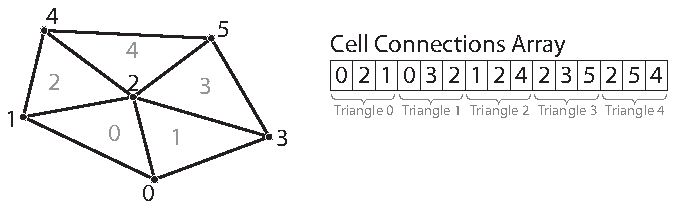
\includegraphics{images/ExplicitCellConnections}
  \caption{An example explicit mesh.}
  \label{fig:ExplicitMesh}
\end{figure}

The \vtkmcont{DataSetBuilderExplicit} class can be used to create data sets
with explicit meshes. \textidentifier{DataSetBuilderExplicit} has several
versions of a method named \textcode{Create}. Generally, these methods take
the shapes, number of indices, and connectivity arrays as well as an array
of point coordinates. These arrays can be given in \textcode{std::vector}
objects, and the data are copied into the \textidentifier{DataSet} created.

The following example creates a mesh like the one shown in
Figure~\ref{fig:ExplicitMesh}.

\vtkmlisting{Creating an explicit mesh with \textidentifier{DataSetBuilderExplicit}.}{CreateExplicitGrid.cxx}

Often it is awkward to build your own arrays and then pass them to
\textidentifier{DataSetBuilderExplicit}. There also exists an alternate
builder class named \vtkmcont{DataSetBuilderExplicitIterative} that allows
you to specify each cell and point one at a time rather than all at once.
This is done by calling one of the versions of \textcode{AddPoint} and one
of the versions of \textcode{AddCell} for each point and cell,
respectively. The next example also builds the mesh shown in
Figure~\ref{fig:ExplicitMesh} except this time using
\textidentifier{DataSetBuilderExplicitIterative}.

\vtkmlisting{Creating an explicit mesh with \textidentifier{DataSetBuilderExplicitIterative}.}{CreateExplicitGridIterative.cxx}

\subsubsection{Add Fields}

In addition to creating the geometric structure of a data set, it is
usually important to add fields to the data. Fields describe numerical data
associated with the topological elements in a cell. They often represent a
physical quantity (such as temperature, mass, or volume fraction) but can
also represent other information (such as indices or classifications).

The easiest way to define fields in a data set is to use the
\vtkmcont{DataSetFieldAdd} class. This class works on
\textidentifier{DataSet}s of any type. It has methods named
\textcode{AddPointField} and \textcode{AddCellField} that define a field
for either points or cells. Every field must have an associated field name.

Both \textcode{AddPointField} and \textcode{AddCellField} are overloaded to
accept arrays of data in different structures. Field arrays can be passed
as standard C arrays or as \textcode{std::vector}s, in which case the data
are copied. Field arrays can also be passed in a
\textidentifier{ArrayHandle}, in which case the data are not copied.

The following (somewhat contrived) example defines fields for a uniform
grid that identify which points and cells are on the boundary of the mesh.

\vtkmlisting{Adding fields to a \textidentifier{DataSet}.}{AddFieldData.cxx}

\index{data~set!Building|)}

\subsection{Cell Sets}
\label{sec:DataSets:CellSets}

\index{cell~set|(}
\index{data~set!cell~set|see{cell~set}}

A cell set determines the topological structure of the data in a data set.
Fundamentally, any cell set is a collection of cells, which typically (but
not always) represent some region in space. 3D cells are made up of points,
edges, and faces. (2D cells have only points and edges, and 1D cells have
only points.) The arrangement of these points, edges, and faces is defined
by the \index{shape}\index{cell~set!shape}\index{cell~shape}\keyterm{shape}
of the cell, which prescribes a specific ordering of each. The basic cell
shapes provided by VTK-m are discussed in detail in
Section~\ref{sec:CellShapeTagsIds} starting on
page~\pageref{sec:CellShapeTagsIds}.

There are multiple ways to express the connections of a cell set, each with
different benefits and restrictions. These different cell set types are
managed by different cell set classes in VTK-m. All VTK-m cell set classes
inherit from \vtkmcont{CellSet}. The two basic types of cell sets are
structured and explicit, and there are several variations of these types.

\subsubsection{Structured Cell Sets}

\index{cell~set!structured|(}
\index{structured~cell~set|(}

A \vtkmcont{CellSetStructured} defines a 1-, 2-, or 3-dimensional grid of
points with lines, quadrilaterals, or hexahedra, respectively, connecting
them. The topology of a \textidentifier{CellSetStructured} is specified by
simply providing the dimensions, which is the number of points in the $i$,
$j$, and $k$ directions of the grid of points. The number of points is
implicitly $i \times j \times k$ and the number of cells is implicitly
$(i-1) \times (j-1) \times (k-1)$ (for 3D grids).
Figure~\ref{fig:CellSetStructured} demonstrates this arrangement.

\begin{figure}
  \centering
  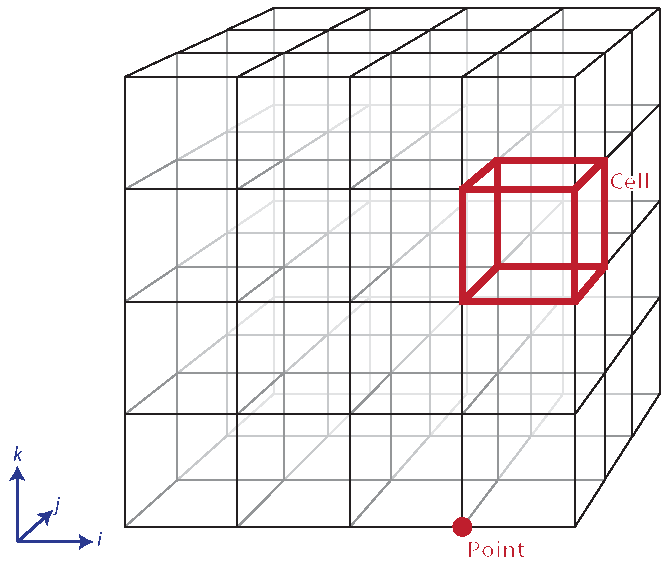
\includegraphics{images/StructuredCellSet}
  \caption{The arrangement of points and cells in a 3D structured grid.}
  \label{fig:CellSetStructured}
\end{figure}

The big advantage of using \vtkmcont{CellSetStructured} to define a cell
set is that it is very space efficient because the entire topology can be
defined by the three integers specifying the dimensions. Also algorithms
can be optimized for \textidentifier{CellSetStructured}'s regular nature.
However, \textidentifier{CellSetStructured}'s strictly regular grid
structure also limits its applicability. A structured cell set can only be
a dense grid of lines, quadrilaterals, or hexahedra. It cannot represent
irregular data well.

Many data models in other software packages, such as the one for VTK, make
a distinction between uniform, rectilinear, and curvilinear grids. VTK-m's
cell sets do not. All three of these grid types are represented by
\textidentifier{CellSetStructured}. This is because in a VTK-m data set the
cell set and the coordinate system are defined independently and used
interchangeably. A structured cell set with uniform point coordinates makes
a uniform grid. A structured cell set with point coordinates defined
irregularly along coordinate axes makes a rectilinear grid. And a
structured cell set with arbitrary point coordinates makes a curvilinear
grid. The point coordinates are defined by the data set's coordinate system,
which is discussed in Section~\ref{sec:DataSets:CoordinateSystems} starting
on page~\pageref{sec:DataSets:CoordinateSystems}.

\index{structured~cell~set|)}
\index{cell~set!structured|)}

\subsubsection{Explicit Cell Sets}

\index{explicit~cell~set|(}
\index{cell~set!explicit|(}

A \vtkmcont{CellSetExplicit} defines an irregular collection of cells. The
cells can be of different types and connected in arbitrary ways. This is
done by explicitly providing for each cell a sequence of points that
defines the cell.

An explicit cell set is defined with a minimum of three arrays. The first
array identifies the shape of each cell. (Cell shapes are discussed in
detail in Section~\ref{sec:CellShapeTagsIds} starting on
page~\pageref{sec:CellShapeTagsIds}.) The second array identifies how many
points are in each cell. The third array has a sequence of point indices
that make up each cell. Figure~\ref{fig:CellSetExplicit} shows a simple
example of an explicit cell set.

\begin{figure}
  \centering
  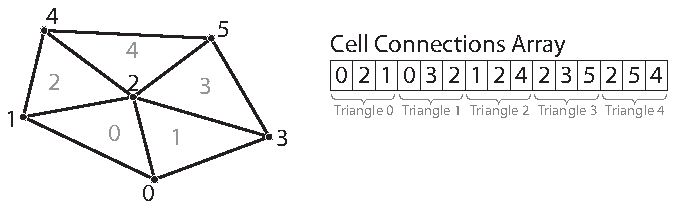
\includegraphics{images/ExplicitCellConnections}
  \caption{Example of cells in a \textidentifier{CellSetExplict} and the
    arrays that define them.}
  \label{fig:CellSetExplicit}
\end{figure}

An explicit cell set may also have other topological arrays such as an
array of offsets of each cell into the connectivity array or an array of
cells incident on each point. Although these arrays can be provided, they
are optional and can be internally derived from the shape, num indices, and
connectivity arrays.

\vtkmcont{ExplicitCellSet} is a powerful representation for a cell set
because it can represent an arbitrary collection of cells. However, because
all connections must be explicitly defined,
\textidentifier{ExplicitCellSet} requires a significant amount of memory to
represent the topology.

\index{cell~set!single~type|(}
\index{explicit~cell~set!single~type|(}
\index{single~type~cell~set|(}

An important specialization of an explicit cell set is
\vtkmcont{CellSetSingleType}. \textidentifier{CellSetSingleType} is an
explicit cell set constrained to contain cells that all have the same shape
and all have the same number of points. So for example if you are creating
a surface that you know will contain only triangles,
\textidentifier{CellSetSingleType} is a good representation for these data.

Using \textidentifier{CellSetSingleType} saves memory because the array of
cell shapes and the array of point counts no longer need to be stored.
\textidentifier{CellSetSingleType} also allows VTK-m to skip some
processing and other storage required for general explicit cell sets.

\index{single~type~cell~set|)}
\index{explicit~cell~set!single~type|)}
\index{cell~set!single~type|)}

\index{cell~set!explicit|)}
\index{explicit~cell~set|)}

\subsubsection{Cell Set Permutations}

\index{permutation~cell~set|(}
\index{cell~set!permutation|(}

A \vtkmcont{CellSetPermutation} rearranges the cells of one cell set to
create another cell set. This restructuring of cells is not done by copying
data to a new structure. Rather, \textidentifier{CellSetPermutation}
establishes a look-up from one cell structure to another. Cells are permuted
on the fly while algorithms are run.

A \textidentifier{CellSetPermutation} is established by providing a mapping
array that for every cell index provides the equivalent cell index in the
cell set being permuted. \textidentifier{CellSetPermutation} is most often
used to mask out cells in a data set so that algorithms will skip over
those cells when running. Note that although
\textidentifier{CellSetPermutation} can mask cells, it cannot mask points.
All points from the original cell set are available in the permuted cell
set regardless of whether they are used.

The following example uses \vtkmcont{CellSetPermutation} with a counting
array to expose every tenth cell. This provides a simple way to subsample a
data set.

\vtkmlisting{Subsampling a data set with \textidentifier{CellSetPermutation}.}{CreateCellSetPermutation.cxx}

\index{cell~set!permutation|)}
\index{permutation~cell~set|)}

\subsubsection{Dynamic Cell Sets}

\index{dynamic~cell~set|(}
\index{cell~set!dynamic|(}

\vtkmcont{DataSet} must hold an arbitrary collection of \vtkmcont{CellSet}
objects, which it cannot do while knowing their types at compile time. To
manage storing \textidentifier{CellSet}s without knowing their types,
\textidentifier{DataSet} actually holds references using
\vtkmcont{DynamicCellSet}.

\textidentifier{DynamicCellSet} is similar in nature to
\textidentifier{DynamicArrayHandle} except that it, of course, holds
\textidentifier{CellSet}s instead of \textidentifier{ArrayHandle}s. The
interface for the two classes is similar, and you should review the
documentation for \textidentifier{DynamicArrayHandle} (in
Section~\ref{sec:DynamicArrayHandle} starting on
page~\pageref{sec:DynamicArrayHandle}) to understand
\textidentifier{DynamicCellSet}.

\vtkmcont{DynamicCellSet} has a method named \textcode{GetCellSet} that
returns a const reference to the held cell set as the abstract
\textidentifier{CellSet} class. This can be used to easily access the
virtual methods in the \textidentifier{CellSet} interface. You can also
create a new instance of a cell set with the same type using the
\textcode{NewInstance} method.

The \textidentifier{DynamicCellSet}\textcode{::IsType()} method can be used
to determine whether the cell set held in the dynamic cell set is of a
given type. If the cell set type is known,
\textidentifier{DynamicCellSet}\textcode{::CastTo()} can be used to safely
downcast the cell set object.

When a typed version of the cell set stored in the
\textidentifier{DynamicCellSet} is needed but the type is not known, which
happens regularly in the internal workings of VTK-m, the
\textcode{CastAndCall} method can be used to make this transition.
\textcode{CastAndCall} works by taking a functor and calls it with the
appropriately cast cell set object.

The \textcode{CastAndCall} method works by attempting to cast to a known
set of types. This set of types used is defined by the macro
\vtkmmacro{VTKM\_DEFAULT\_CELL\_SET\_LIST\_TAG}, which is declared in
\vtkmheader{vtkm/cont}{CellSetListTag.h}. This list can be overridden
globally by defining the \vtkmmacro{VTKM\_DEFAULT\_CELL\_SET\_LIST\_TAG}
macro \emph{before} any VTK-m headers are included.

The set of types used in a \textcode{CastAndCall} can also be changed only
for a particular instance of a dynamic cell set by calling its
\textcode{ResetCellSetList}. This method takes a list of cell types and
returns a new dynamic array handle of a slightly different type that will
use this new list of cells for dynamic casting.

\index{cell~set!dynamic|)}
\index{dynamic~cell~set|}

\subsubsection{Blocks and Assemblies}

Rather than just one cell set, a \vtkmcont{DataSet} can hold multiple cell
sets. This can be used to construct multiblock data structures or
assemblies of parts. Multiple cell sets can also be used to represent
subsets of the data with particular properties such as all cells filled
with a material of a certain type. Or these multiple cells might represent
particular features in the data, such as the set of faces representing a
boundary in the simulation.

\subsubsection{Zero Cell Sets}

It is also possible to construct a \vtkmcont{DataSet} that contains no cell
set objects whatsoever. This can be used to manage data that does not
contain any topological structure. For example, a collection of series that
come from columns in a table could be stored as multiple fields in a data
set with no cell set.

\index{cell~set|)}

\subsection{Fields}
\label{sec:DataSets:Fields}

\index{field|(}
\index{data~set!field|see{field}}

A field on a data set provides a value on every point in space on the mesh.
Fields are often used to describe physical properties such as pressure,
temperature, mass, velocity, and much more. Fields are represented in a
VTK-m data set as an array where each value is associated with a particular
element type of a mesh (such as points or cells). This association of field
values to mesh elements and the structure of the cell set determines how
the field is interpolated throughout the space of the mesh.

Fields are manged by the \vtkmcont{Field} class. \textidentifier{Field}
holds its data with a \textidentifier{DynamicArrayHandle}, which itself is
a container for an \textidentifier{ArrayHandle}. \textidentifier{Field}
also maintains the association and, optionally, the name of a cell set for
which the field is valid.

The data array can be retrieved as a \textidentifier{DynamicArrayHandle}
using the \textcode{GetData} method of \textidentifier{Field}.
\textidentifier{Field} also has a convenience method named
\textcode{GetBounds} that finds the range of values stored in the field
array.

\index{field|}

\subsection{Coordinate Systems}
\label{sec:DataSets:CoordinateSystems}

\index{coordinate~system|(}
\index{data~set!coordinate~system|see{coordinate~system}}

A coordinate system determines the location of a mesh's elements in space.
The spatial location is described by providing a 3D vector at each point
that gives the coordinates there. The point coordinates can then be
interpolated throughout the mesh.

Coordinate systems are managed by the \vtkmcont{CoordinateSystem} class. In
actuality, a coordinate system is just a field with a special meaning, and
so the \textidentifier{CoordinateSystem} class inherits from the
\textidentifier{Field} class. \textidentifier{CoordinateSystem} constrains
the field to be associated with points and typically has 3D floating point
vectors for values.

It is typical for a \textidentifier{DataSet} to have one coordinate system
defined, but it is possible to define multiple coordinate systems. This is
helpful when there are multiple ways to express coordinates. For example,
positions in geographic may be expressed as Cartesian coordinates or as
latitude-longitude coordinates. Both are valid and useful in different
ways.

It is also valid to have a \textidentifier{DataSet} with no coordinate
system. This is useful when the structure is not rooted in physical space.
For example, if the cell set is representing a graph structure, there might
not be any physical space that has meaning for the graph.

\index{coordinate~system|)}

\index{data~set|)}

\section{Timers}
\label{sec:Timers}

\index{timer|(}

It is often the case that you need to measure the time it takes for an
operation to happen. This could be for performing measurements for
algorithm study or it could be to dynamically adjust scheduling.

Performing timing in a multi-threaded environment can be tricky because
operations happen asynchronously. In the VTK-m control environment timing
is simplified because the control environment operates on a single
thread. However, operations invoked in the execution environment may run
asynchronously to operations in the control environment.

To ensure that accurate timings can be made, VTK-m provides a
\vtkmcont{Timer} class that is templated on the device adapter to provide
an accurate measurement of operations that happen on the device. If not
template parameter is provided, the default device adapter is used.

The timing starts when the \textidentifier{Timer} is constructed. The time
elapsed can be retrieved with a call to the \textcode{GetElapsedTime}
method. This method will block until all operations in the execution
environment complete so as to return an accurate time. The timer can be
restarted with a call to the \textcode{Reset} method.

\fix{This example needs to be updated when something interesting can be
  invoked.}

\vtkmlisting{Using \protect\vtkmcont{Timer}.}{Timer.cxx}

\index{timer|)}

\section{Error Handling}
\label{sec:ErrorHandlingControl}

\index{errors|(}

VTK-m uses exceptions to report errors. All exceptions thrown by VTK-m will
be a subclass of \vtkmcont{Error}. For simple error reporting, it is
possible to simply catch a \vtkmcont{Error} and report the error message
string reported by the \textcode{GetMessage} method.

\vtkmlisting{Simple error reporting.}{CatchingErrors.cxx}

There are several subclasses to \vtkmcont{Error}. The specific subclass
gives an indication of the type of error that occured when the exception
was thrown. Catching one of these subclasses may help a program better
recover from errors.
\begin{description}
\item[\vtkmcont{ErrorControlAssert}] \index{assert} \index{errors!assert}
  Thrown when an assertion fails, meaning a VTK-m operation reached an
  unexpected state. The header file \vtkmheader{vtkm/cont}{Assert.h}
  defines a macro named \vtkmmacro{VTKM\_ASSERT\_CONT} that behaves much
  like the POSIX C assert macro except that a
  \textidentifier{ErrorControlAssert} is thrown rather than killing the
  application outright.
\item[\vtkmcont{ErrorControlBadAllocation}] Thrown when there is a problem
  accessing or manipulating memory. Often this is thrown when an allocation
  fails because there is insufficient memory, but other memory access
  errors can cause this to be thrown as well.
\item[\vtkmcont{ErrorControlBadType}] Thrown when VTK-m attempts to perform
  an operation on an object that is of an incompatible type.
\item[\vtkmcont{ErrorControlBadValue}] Thrown when a VTK-m function or
  method encounters an invalid value that inhibits progress.
\item[\vtkmcont{ErrorExecution}] \index{errors!execution~environment} Throw
  when an error is signaled in the execution environment for example when a
  worklet is being executed.
\item[\vtkmcont{ErrorControlInternal}] Thrown when VTK-m detects an
  internal state that should never be reached. This error usually indicates
  a bug in VTK-m or, at best, VTK-m failed to detect an invalid input it
  should have.
\item[\vtkmio{ErrorIO}] Thrown by a reader or writer when a file error is
  encountered.
\end{description}

\index{errors|)}

\index{environment!control|)}
\index{control~environment|)}



\chapter{Execution Environment}
\label{chap:ExecutionEnvironment}

\fix{Write this.}

\chapter{OpenGL Interoperability}
\label{chap:OpenGLInteroperability}

\chapter{Coding Conventions}
\label{chap:CodingConventions}


\begin{flushleft}
  \clearpage
  \lhead[]{}
  \rhead[]{}
  \phantomsection
  \addcontentsline{toc}{chapter}{Index}
  \printindex
\end{flushleft}

% -*- latex -*-

\begin{SANDdistribution}[NM]
  % External Addresses
  %% \SANDdistExternal{1}{Lucy Nowell\\ U.S. Department of Energy\\ SC-21\\ 19901 Germantown Road\\ Germantown, MD 20874-1290}
  %% \SANDdistExternal{1}{Teresa Beachley\\ U.S. Department of Energy\\ SC-21\\ 19901 Germantown Road\\ Germantown, MD 20874-1290}
  %% \SANDdistExternal{1}{Berk Geveci\\ Kitware, Inc.\\ 28 Corporate Drive\\ Clifton Park, NY 12065}
  %% \SANDdistExternal{1}{Robert Maynard\\ Kitware, Inc.\\ 28 Corporate Drive\\ Clifton Park, NY 12065}
  %% \SANDdistExternal{1}{Kwan-Liu Ma\\ Department of Computer Science\\ 2063 Kemper Hall\\ University of California-Davis\\ One Shields Avenue\\ Davis, CA 95616-8562}

  \bigskip

  % Internal Addresses
  \SANDdistInternal{1}{1326}{Kenneth Moreland}{1461}
  \SANDdistInternal{1}{1327}{Ron Oldfield}{01461}
\end{SANDdistribution}


\end{document}
